\documentclass[11pt]{article}
\usepackage{amsmath,amssymb,amsthm,mathtools}
\usepackage[margin=1in]{geometry}
\usepackage{graphicx}
\usepackage{hyperref}

\theoremstyle{plain}
\newtheorem{theorem}{Theorem}[section]
\newtheorem{proposition}[theorem]{Proposition}
\newtheorem{lemma}[theorem]{Lemma}
\newtheorem{corollary}[theorem]{Corollary}
\newtheorem{conjecture}[theorem]{Conjecture}
\theoremstyle{definition}
\newtheorem{definition}[theorem]{Definition}
\newtheorem{assumption}[theorem]{Assumption}
\theoremstyle{remark}
\newtheorem{remark}[theorem]{Remark}

\DeclareMathOperator{\Var}{Var}\DeclareMathOperator{\Cov}{Cov}
\DeclareMathOperator{\Corr}{Corr}\DeclareMathOperator{\cum}{cum}
\DeclareMathOperator{\supp}{supp}
\newcommand{\Z}{\mathbb{Z}}\newcommand{\R}{\mathbb{R}}\newcommand{\N}{\mathbb{N}}
\newcommand{\E}{\mathbb{E}}\newcommand{\PP}{\mathbb{P}}\newcommand{\dd}{\,\mathrm{d}}
\newcommand{\To}{\Rightarrow}\newcommand{\so}{\mathfrak{so}}
\newcommand{\sutwo}{\mathfrak{sl}_2}\newcommand{\Lt}{\widetilde{\mathcal L}}
\newcommand{\ip}[2]{\langle #1,#2\rangle_\nu}\newcommand{\bone}{\mathbf 1}
\newcommand{\eps}{\varepsilon}\newcommand{\Exp}{\mathrm{Exp}}
\newcommand{\cC}{\mathcal C}\newcommand{\cS}{\mathcal S}\newcommand{\cF}{\mathcal F}
\newcommand{\cL}{\mathcal L}\newcommand{\cO}{\mathcal O}\newcommand{\cE}{\mathcal E}

\title{\bf Fluctuations of the type D ASEP:\\
decoupling in two universality classes}
\author{(working draft --- full version)}
\date{\today}

\begin{document}
\maketitle

\begin{abstract}
The type D ASEP is a two--species interacting particle system on $\Z$, the
$n\to\infty$ degeneration of the $U_q(\so_{2n+2})$ exclusion process of Kuan, Landry,
Lin, Park and Zhou, in which two separately conserved species hop, bind into a
composite ``bound pair'', and split. The binding interaction couples the two species
at the microscopic level as directly as a conservative dynamics can; the question we
ask is whether that coupling survives to the scale of the fluctuations. We analyse the
density and current fluctuations in two scaling regimes and prove that in both the two
species \emph{decouple} --- but for two different reasons.

In the critically weak--asymmetry (Edwards--Wilkinson) regime $q=1-c/N^2$ we prove
that the two density fluctuation fields \emph{decouple}: each converges to a linear
stochastic heat equation, with no cross--coupling in either the drift or the noise,
the limiting noises having vanishing cross--correlation (Theorem~\ref{thm:ewmain}).
The proof is self--contained modulo the classical single--species fluctuation result:
the drift reduces, via the exact current decoupling (Proposition~\ref{prop:decouple}),
to an autonomous single--species WASEP, while the cross--noise cancellation is controlled
by a two--particle dual kernel bound
(Theorem~\ref{thm:kernel}) proved here in full, including the underlying
one--dimensional local limit estimates (\S\ref{sec:lclt}). The inter--species coupling the model nonetheless exhibits is
shown to be purely an initial--condition effect, computed in closed form through the
two--particle dual (Theorem~\ref{thm:closed}): a position correlation
$(1-e^{-4c})/(4c)$ and a Bessel--Struve form for the $q$--Krawtchouk observable, both
with $1/c$ tails.

In the fixed--$q$ (Kardar--Parisi--Zhang) regime an exact current--decoupling identity,
valid at every $n$ (Propositions~\ref{prop:decouple}, \ref{prop:decouplen}), makes each
species' current an autonomous single--species ASEP, hence Tracy--Widom for every $n$
--- proving a conjecture of \cite{REU}. Here too the species decouple: we prove an
exact contact representation for the joint $q$--Laplace observable ---
$\Cov(q^{2N_1},q^{2N_2})$ is a weighted sum of connected two--particle dual hitting
probabilities, vanishing identically without the binding (Theorem~\ref{thm:cov}) ---
while for the linear currents simulations give
$\Cov(N_1,N_2)=(0.099\pm0.003)\sqrt s$ at $q=\tfrac12$, so that
$\Corr(N_1,N_2)\asymp s^{-1/6}\to0$ (Conjecture~\ref{conj:cov}). The common engine is the $q$--Krawtchouk orthogonal
self--duality, together with the fact --- which we make precise --- that the
inter--species coupling is invisible to every equilibrium transport coefficient, so
that in both regimes what remains of it is a transient, initial--condition--driven
correlation rather than a feature of the limiting law.
\end{abstract}

{\small\tableofcontents}

\section{Introduction}\label{sec:intro}

When several conserved species share one exclusion dynamics, the basic question is
whether they interact at the scale of their fluctuations: do the density and current
fields couple in the scaling limit, or does each species behave as an autonomous
single--species process? Coupling is the generic expectation, and it is what produces
the rich behaviour of multi--species models --- off--diagonal transport coefficients,
distinct characteristic speeds, and the non--Gaussian or non--Tracy--Widom joint laws
that come with them. This paper studies a model in which the answer runs the other way.
The two species are not merely placed on a common lattice: they are dynamically
\emph{fused} into composite pairs and later \emph{split}, so any inter--species
coupling has a direct microscopic channel through which to act. Yet in two distinct
scaling limits the two components decouple completely, and our aim is to locate exactly
where the interaction goes --- and why it never reaches the limiting law.

\subsection{The model}\label{sec:intromodel}
Fix $q\in(0,1)$. The \emph{type D ASEP} was introduced by Kuan, Landry, Lin, Park and
Zhou \cite{KLLPZ}, who constructed it from the quantum groups $U_q(\so_6)$ and
$U_q(\so_8)$ ($n=2,3$ in $\so_{2n+2}$, Cartan type $D$); the construction has been
extended to $U_q(\so_{10})$ \cite{RSL}, and the explicit rate matrix (displayed for
general $n$ in \cite[\S2.1]{REU}) makes sense for every $n\in\N$. It is a
continuous--time Markov process of two conserved species on $\Z$ which, beyond
hopping, may bind into a composite \emph{bound pair} and later split. This binding is
what makes the model a stringent test of decoupling: the two species are genuinely
interacting, not two independent copies sharing the exclusion rule. Blyschak, Burke,
Kuan, Li, Ustilovsky and Zhou \cite{REU} established an orthogonal $q$--Krawtchouk
self--duality for $n=2,3$ and conjectured it for all $n$; we verify it at the
$n=\infty$ degeneration used here (Theorem~\ref{thm:dual}(ii)). The duality is the
analytic engine of this paper: it reduces every fluctuation question to a computation
with a handful of dual particles.

We work in the limit $n\to\infty$, in which (after rescaling time by $q^{2n}$) the
dynamics closes on the four local states $\{0,1,2,3\}$ at each site: empty, species
$1$, species $2$, and a bound pair carrying one particle of each species. With
$\eta_{i,x}\in\{0,1\}$ the occupation of species $i$ at $x$, so that
$\omega_x=\eta_{1,x}+2\eta_{2,x}$, and with $\eps:=1-q^2$, the nonzero
nearest--neighbour rates are
\begin{equation}\label{eq:rates}
\begin{aligned}
&(1,0)\!\to\!(0,1):1, &&(0,1)\!\to\!(1,0):q^2, &&(2,0)\!\to\!(0,2):1, &&(0,2)\!\to\!(2,0):q^2,\\
&(3,0)\!\to\!(0,3):1, &&(0,3)\!\to\!(3,0):q^4, &&(0,3)\!\to\!(1,2):q^2\eps, &&(0,3)\!\to\!(2,1):q^2\eps,\\
&(1,2)\!\to\!(0,3):\eps, &&(1,2)\!\to\!(2,1):q^2, &&(2,1)\!\to\!(0,3):\eps, &&(2,1)\!\to\!(1,2):q^2,
\end{aligned}
\end{equation}
together with mixed hops $(3,1)\!\leftrightarrow\!(1,3)$ and
$(3,2)\!\leftrightarrow\!(2,3)$ at rate $1$ right, $q^2$ left, in which a single
species slides past a bound pair. The two species numbers are conserved. For finite
$n$ a single species is a usual ASEP with rates $q^{\pm1}\beta_n$,
$\beta_n=q^{1-2n}+q^{2n-1}$, so $n$ enters the single--species dynamics only as a time
rescaling.

\subsection{Results}\label{sec:introresults}
Decoupling might hold for one reason in one universality class and fail in another, so
we test it in the two canonical fluctuation classes of driven diffusive systems. We
treat two scalings. \emph{(A) The Edwards--Wilkinson regime}: asymmetry tuned to
the diffusive rate $q=q_N=1-c/N^2$, under diffusive space--time scaling, at any pair of
densities $(\rho_1,\rho_2)$. \emph{(B) The Kardar--Parisi--Zhang
regime}: $q\in(0,1)$ fixed, the integrated currents $N_1(s),N_2(s)$ across the origin
from the step initial condition, at a single time $s$. Our principal theorems are
Theorems~\ref{thm:ewmain}, \ref{thm:closed} (regime A) and \ref{thm:marg},
\ref{thm:cov} (regime B), proved in \S\S\ref{sec:ew}--\ref{sec:tw}. The logical
backbone common to both regimes --- the reversible measure and orthogonal duality
(\S\ref{sec:model}), the exact current decoupling and vanishing transport
coefficients (\S\ref{sec:decouple}), and a local CLT for the dual coordinates
(\S\ref{sec:lclt}) --- is developed first.

\subsection{Relation to previous work}\label{sec:introlit}
Regime~(A) belongs to the nonlinear fluctuation theory of weakly asymmetric systems and
the passage to stochastic Burgers/KPZ, due to Gon\c{c}alves and Jara \cite{GJ}, with
uniqueness by Gubinelli and Perkowski and spectral--gap--free refinements by
Gon\c{c}alves, Jara and Simon \cite{GJS}. The few--body estimates we need we obtain
through the \emph{orthogonal polynomial duality} method of Ayala, Carinci and Redig
\cite{ACR,ACR2}, which reduces them to a decay bound on the few--particle dual kernel. In
our setting the exact current decoupling (Proposition~\ref{prop:decouple}) makes the
drift an autonomous single--species WASEP, so the duality enters only for the
inter--species cross--noise, controlled by the type D two--particle kernel bound of
\S\ref{sec:kernel}; the would--be slow internal mode of the bound pair never couples to
the species current at all (Proposition~\ref{prop:sym}).

For regime~(B), the single--species Tracy--Widom asymptotics are
Borodin--Corwin--Sasamoto \cite{BCS}; the exact $q$--Laplace decoupling identity
(Theorem~\ref{thm:cov}) is to our knowledge new, and the Tracy--Widom marginals at
every $n$ (Theorem~\ref{thm:marg}) prove the conjecture of \cite[\S3.1.1]{REU}.

The structural point is what distinguishes type D from other multi--species models. Its
inter--species coupling is invisible to both the static compressibility and the dynamic
mobility, so what remains of it is a transient, initial--condition--driven correlation
rather than a transport effect. This sets type D apart from the multi--species models
with genuine off--diagonal transport coefficients (e.g.\ multi--species stirring, with
multinomial mobility) and from the distinct--velocity two--species KPZ decouplings:
type D sits instead at the \emph{umbilic point}, where the characteristic velocities
coincide and both of those mechanisms are unavailable. We are not aware of another
model combining diffusive (EW) class, diagonal compressibility, vanishing
cross--mobility, and a nonzero shared--source inter--species correlation with a
$\rho(c)\sim1/c$ crossover.

\subsection{Organisation}\label{sec:introorg}
Section~\ref{sec:model} fixes the generator, reversible measure, and orthogonal
self--duality. Section~\ref{sec:decouple} proves the exact current decoupling and the
vanishing static/dynamic cross coefficients. Section~\ref{sec:lclt} proves the
random--walk local CLTs used throughout. Section~\ref{sec:kernel} proves the
two--particle dual kernel bound. Section~\ref{sec:ew} proves the decoupled
Edwards--Wilkinson limit. Section~\ref{sec:cross} proves the initial--condition
crossover. Section~\ref{sec:tw} proves the Tracy--Widom marginals at every $n$ and
the exact $q$--Laplace decoupling of the two currents, and states the linear
covariance asymptotics as a conjecture. Section~\ref{sec:phase} records the
asymmetry--exponent phase picture and further numerical observations.
Section~\ref{sec:disc} discusses open problems. Physical interpretation is confined to
remarks.

\section{The model, the measure, and the duality}\label{sec:model}

We first record the three structures on which the entire analysis rests: the generator,
the reversible product measure, and the orthogonal $q$--Krawtchouk self--duality. The
duality is the decisive one --- it is what turns a question about the full interacting
field into a question about one or two dual particles, and both regimes are ultimately
solved by the same few--body computation.

For a local function $f$ of $\eta\in\{0,1,2,3\}^\Z$ the generator is
\begin{equation}\label{eq:gen}
  \cL f(\eta)=\sum_{x\in\Z}\sum_{(a,b)\to(a',b')}
   r\big((a,b)\to(a',b')\big)\,\bone\{\omega_x=a,\omega_{x+1}=b\}
   \big[f(\eta^{x,x+1}_{a'b'})-f(\eta)\big],
\end{equation}
the inner sum over the transitions of \eqref{eq:rates}, $\eta^{x,x+1}_{a'b'}$ denoting
$\eta$ with $(\omega_x,\omega_{x+1})$ reset to $(a',b')$. The finite--$n$ rate matrix
is displayed in \cite[\S2.1]{REU} (constructed from the quantum group for $n=2,3$ in
\cite{KLLPZ}); after the time rescaling by $q^{2n}$ its entrywise $n\to\infty$ limit
is \eqref{eq:rates}, which one checks directly to be a Markov generator with the
stated conservation laws for every $q\in(0,1)$.

\begin{proposition}[reversible measure; {\cite[Prop.~1.3]{KLLPZ}},{\cite[\S3.1]{REU}}]
\label{prop:measure}
The type D ASEP is reversible with respect to the product blocking measure
\begin{equation}\label{eq:nu}
  \nu(\eta)=\mu_{\alpha_1}(\eta_1)\,\mu_{\alpha_2}(\eta_2),\qquad
  \mu_\alpha(\xi)=\prod_{x\in\Z}\alpha^{\xi_x}q^{-2x\xi_x}\quad(\alpha>0),
\end{equation}
a product over both sites and species, carrying the $q^{-2x}$ density tilt, the two
species independent.
\end{proposition}

\begin{lemma}[local detailed balance]\label{lem:db}
For $\nu$ and adjacent sites $(x,x+1)$, the unnormalised two--point weights satisfy
\begin{equation}\label{eq:dbrel}
  \nu(0,3)=q^{-4}\nu(3,0),\qquad \nu(1,2)=\nu(2,1)=q^{-2}\nu(3,0).
\end{equation}
\end{lemma}
\begin{proof}
By \eqref{eq:nu} the weight on $\{x,x+1\}$ factorises over the two sites and two
species; a species--$i$ particle at site $y$ contributes $\alpha_i q^{-2y}$. Moving the
bound pair from $x$ to $x+1$ multiplies the weight by $q^{-2}\cdot q^{-2}=q^{-4}$;
moving one species--$1$ particle from $x$ to $x+1$ and one species--$2$ particle from
$x+1$ to $x$ leaves a single $q^{-2}$ deficit. These are precisely the
detailed--balance identities of \eqref{eq:rates} for $\nu$.
\end{proof}

\begin{remark}[parameter range and the locked limit]\label{rem:range}
Although $n$ indexes finite--dimensional representations of $\so_{2n+2}$, the
finite--$n$ generator of \cite[\S2.1]{REU} extends analytically in $n$ and remains a
bona fide Markov generator for a range of \emph{negative} $n$: the binding rates
$(1,2)\to(3,0)$, $(3,0)\to(1,2)$ are the constraints, both proportional to
$2-q^{2n-2}(1-q^2)$ and hence vanishing at
$n_{\mathrm{crit}}=\log\!\big(2q^2/(1-q^2)\big)/(2\log q)$, so the process is stochastic
for $n>n_{\mathrm{crit}}$, with $n_{\mathrm{crit}}<0$ exactly when $q>1/\sqrt3$ (i.e.\
$2q^2/(1-q^2)>1$). At
$q=1$ the split/merge rates vanish, bound pairs never break, $N_1\equiv N_2$, and the
species are perfectly locked.
\end{remark}

\subsection{The orthogonal \texorpdfstring{$q$}{q}--Krawtchouk self--duality}
Each site holds at most one particle of each species, so the single--site,
single--species marginal is the two--point specialisation of the $q$--Krawtchouk
family. With local fugacity $t_x:=\alpha q^{-2x}$ and density $\rho_x=t_x/(1+t_x)$,
the degree--$\le1$ orthogonal polynomials of $\mu_\alpha$ are
\begin{equation}\label{eq:d1}
  \kappa_0(\eta_x)\equiv1,\qquad
  \kappa_1(\eta_x)=\frac{(1+t_x)\eta_x-t_x}{\sqrt{t_x}}
  =\frac{\eta_x-\rho_x}{\sqrt{\rho_x(1-\rho_x)}}.
\end{equation}

\begin{definition}[orthonormal local basis]\label{def:D}
For a dual configuration $\xi$ specifying which (site, species) pairs carry a dual
particle, set
\begin{equation}\label{eq:Dfac}
  D^{\mathrm{loc}}(\xi,\eta)=\prod_{(x,i):\,\xi_{i,x}=1}\kappa_1(\eta_{i,x}),
\end{equation}
a polynomial in $\eta$ of degree $|\xi|$ (the dual mass). By the product structure of
$\nu$ and the single--site orthonormality of \eqref{eq:d1}, the family
$\{D^{\mathrm{loc}}(\xi,\cdot)\}$ is orthonormal in $L^2(\nu)$. It is the natural
basis for the fluctuation fields: mass--one elements are the centred density fields,
and the different--species mass--two element at one site is the bound--pair mode.
\end{definition}

\begin{remark}[$D^{\mathrm{loc}}$ is \emph{not} the duality function]\label{rem:norm}
An earlier version of this draft asserted self--duality with respect to
\eqref{eq:Dfac}. That is false, for a structural reason: every
$\int D^{\mathrm{loc}}(\xi,\cdot)^2\dd\nu=1$, and reversibility makes
$\langle P_tD^{\mathrm{loc}}_\xi,D^{\mathrm{loc}}_{\xi'}\rangle_\nu$ a symmetric
matrix, so duality with respect to \eqref{eq:Dfac} would force a symmetric dual
transition kernel --- impossible for the asymmetric, sticky--origin dual particle
dynamics. (We also verified the failure directly: on two and three sites the
interlacing $\cL D^{\mathrm{loc}}=D^{\mathrm{loc}}\cL^{\mathsf T}$ fails by $O(1)$
margins at generic parameters.) The true duality function of \cite{REU} carries
nonlocal counting factors, as follows.
\end{remark}

\begin{theorem}[orthogonal $q$--Krawtchouk self--duality]\label{thm:dual}
For configurations $\eta,\xi$ and $i\in\{1,2\}$ let $N^-_{x-1}(\xi_i)$ be the number
of species--$i$ dual particles strictly to the left of $x$ and $N^+_{x+1}(\eta_i)$
the number of species--$i$ particles of $\eta$ strictly to the right of $x$, and set
\begin{equation}\label{eq:Dreu}
  D_{\alpha_1,\alpha_2}(\xi,\eta)\ =\ \prod_{i=1,2}\ \prod_{x:\,\xi_{i,x}=\eta_{i,x}=1}
  \Big(1-\frac{q^{2\left(x-N^-_{x-1}(\xi_i)+N^+_{x+1}(\eta_i)\right)}}{\alpha_i}\Big),
\end{equation}
the two--point specialisation of the $q$--Krawtchouk product of
\cite[Thm.~3.1]{REU}.
\textup{(i)} \cite[Thm.~3.1]{REU}: for parameters $(q,n,\delta)=(q,2,0)$ and
$(q,3,0)$, the type D ASEP is self--dual with respect to \eqref{eq:Dreu}.
\textup{(ii)} At $n=\infty$, i.e.\ for the rates \eqref{eq:rates}: the two--site
interlacing $\cL D=D\cL^{\mathsf T}$ holds identically in $(q,\alpha_1,\alpha_2)$ ---
a finite rational identity, which we have verified by computer algebra --- and the
induction in the proof of \cite[Thm.~3.1, eqs.~(16)--(19)]{REU}, which uses only the
two--site case and the fugacity--shift covariance of \eqref{eq:Dreu}, extends it to
any number of sites. This settles the $n=\infty$ degeneration of the conjecture of
\cite[Rmk.~4]{REU} that the duality holds for all $n$. In the lineage of orthogonal
stochastic dualities from $U_q$--representations \cite{Groenevelt,CGRS}, this is the
type D instance.
\end{theorem}

\begin{corollary}[triangular degeneration]\label{cor:tri}
Self--duality with respect to \eqref{eq:Dreu} holds identically in
$(\alpha_1,\alpha_2)$, hence coefficient--wise in $\alpha_1^{-1},\alpha_2^{-1}$; and
since the dual generator preserves the particle numbers $(|\xi_1|,|\xi_2|)$, the
coefficients of $\alpha_1^{-|\xi_1|}\alpha_2^{-|\xi_2|}$, glued across the dual
sectors, again form a duality matrix. This extraction yields self--duality with
respect to the \emph{triangular} function
\begin{equation}\label{eq:Dtri}
  D^{\mathrm{tri}}(\xi,\eta)\ =\ \bone\{\xi\subseteq\eta\}\,
  \prod_{i=1,2}\ \prod_{x:\,\xi_{i,x}=1}
  q^{2\left(x-N^-_{x-1}(\xi_i)+N^+_{x+1}(\eta_i)\right)},
\end{equation}
the type D analogue of the Sch\"utz and Borodin--Corwin--Sasamoto $q$--exponential
dualities \cite{Schutz,BCS}. On configurations $\eta$ with finitely many particles to
the right --- in particular on the step initial condition and its evolution --- the
factors of \eqref{eq:Dtri} are uniformly bounded for each fixed dual mass, and
\eqref{eq:Dtri} is the form of the duality used in \S\ref{sec:tw}.
\end{corollary}

\begin{lemma}[duality covariance; {\cite[Lem.~2.1]{ACR}}]\label{lem:acr}
Let $\{D(\xi,\cdot)\}$ be a family of duality functions for the process which is
orthogonal in $L^2(\varpi)$ for some measure $\varpi$,
$\int D(\xi,\eta)D(\xi',\eta)\dd\varpi=\delta_{\xi,\xi'}a(\xi)$. Then for all
$\xi,\xi'$ and $t\ge0$,
\[
  \int \E_\eta[D(\xi,\eta_t)]\,D(\xi',\eta)\dd\varpi(\eta)=p_t(\xi,\xi')\,a(\xi').
\]
\end{lemma}
\begin{proof}
Insert the duality identity
$\E_\eta[D(\xi,\eta_t)]=\sum_{\xi''}p_t(\xi,\xi'')D(\xi'',\eta)$, multiply by
$D(\xi',\eta)$, and integrate against $\varpi$. By orthogonality
$\int D(\xi'',\eta)D(\xi',\eta)\dd\varpi=\delta_{\xi'',\xi'}a(\xi')$, so only
$\xi''=\xi'$
survives. The interchange of sum and integral is justified by the finite mass of
$\xi$ (only finitely many $\xi''$ are reachable in the particle--conserving dual).
\end{proof}

\begin{remark}[the exact orthogonality relation]\label{rem:orthstatus}
The precise orthogonality satisfied by the type D duality functions is the
two--point, two--species specialisation of \cite[Thm.~3.2]{CFG20}, the
single--species input cited in \cite[\S3.1]{REU}. On a finite lattice $\Lambda$ of
$|\Lambda|$ sites define the \emph{sector--reweighted} blocking measure and norm
functions ($N=N(\zeta)$ the particle number, all up to normalisation)
\begin{equation}\label{eq:omegadef}
  \varpi_\alpha(\zeta)\ \propto\ \mu_\alpha(\zeta)\,q^{N(N-1)}\,
  \big(\alpha q^{2N-2|\Lambda|};q^2\big)_\infty,\quad
  g_\alpha(\zeta)\ \propto\ q^{2N(N-1)}
  \big(\alpha q^{2N-2|\Lambda|};q^2\big)_\infty\big(\alpha q^{-2N};q^2\big)_\infty,
\end{equation}
with window $\alpha\in(0,q^{2|\Lambda|})$, and let $\bar D$ denote \eqref{eq:Dreu}
read with the \emph{process} configuration in the $N^-$ slot and the dual in the
$N^+$ slot,
\[
  \bar D(\xi,\eta)=\prod_{i=1,2}\ \prod_{x:\,\xi_{i,x}=\eta_{i,x}=1}
  \Big(1-\frac{q^{2\left(x-N^-_{x-1}(\eta_i)+N^+_{x+1}(\xi_i)\right)}}{\alpha_i}\Big);
\]
transposing the interlacing of Theorem~\ref{thm:dual}(ii), $\bar D$ is again a
self--duality function. Then
\begin{equation}\label{eq:orthexact}
  \sum_\eta \varpi_{\alpha_1}(\eta_1)\,\varpi_{\alpha_2}(\eta_2)\,
  \bar D(\xi,\eta)\,\bar D(\xi',\eta)\ =\ \delta_{\xi,\xi'}\,a(\xi),\qquad
  a(\xi)=\prod_{i=1,2}\frac{g_{\alpha_i}(\xi_i)}{\varpi_{\alpha_i}(\xi_i)},
\end{equation}
which we have verified to machine precision for the $n=\infty$ rates on two and
three sites (off--diagonals and the norm formula). Three observations. (i) The
reweighting in \eqref{eq:omegadef} depends only on the conserved particle numbers,
so $\varpi:=\varpi_{\alpha_1}\otimes\varpi_{\alpha_2}$ is again reversible, and
Lemma~\ref{lem:acr} applies with $(\varpi,\bar D,a)$. (ii) In the orientation
$\bar D$ the process enters through the \emph{left} counts $N^-(\eta_i)$, which are
almost surely finite under $\nu$ on $\Z$: the degeneration that affects
\eqref{eq:Dreu} in infinite volume (where $q^{2N^+(\eta)}=0$ a.s.) does not occur ---
the resolution is to transpose the slots, not to reflect the lattice, which is
impossible (the reflected generator fails the interlacing, consistently with the
reflection corresponding to the non--stochastic continuation $n<n_{\mathrm{crit}}$
of Remark~\ref{rem:range}). (iii) In the regime (A) scaling, $q=1-c/N^2$ on
$|\Lambda|=O(N)$ sites, the window is asymptotically $\alpha_i<1$, i.e.\ both
densities below $\tfrac12$; the case of both densities above $\tfrac12$ follows by
the particle--hole--plus--reflection symmetry of \eqref{eq:rates} (which flips both
species), while the mixed case $\rho_1<\tfrac12<\rho_2$ is \emph{not} reached by the
window and is deferred (e.g.\ via the signed--measure version of the orthogonality
noted in \cite[Rmk.\ after Thm.~3.2]{CFG20}). The reweighting
is bounded above and below by constants (Lemma~\ref{lem:sector}). The remaining
infinite--volume step --- replacing $[-KN,KN]$ by $\Z$ in the correlation functions
--- is deferred to the final version. In regime (B) we use the triangular duality
of Corollary~\ref{cor:tri} instead.
\end{remark}

\noindent Lemma~\ref{lem:acr} reduces every space--time correlation of degree--$k$
fields to a single $k$--particle dual kernel evaluation --- the orthogonal--duality
reduction of few--body correlations of \cite{ACR,ACR2}, and the mechanism that makes the
fluctuation theory a few--body problem. In this paper it is applied at $k=2$, to the
inter--species cross--noise (\S\ref{sec:ew}).

\section{Exact current decoupling and vanishing transport coefficients}\label{sec:decouple}

The structural fact behind every decoupling result in this paper is elementary and
exact, holding at the level of the microscopic rates: at $n=\infty$ each species'
current does not see the other. We prove this first (Proposition~\ref{prop:decouple}),
then draw its two consequences --- that each marginal is an autonomous single--species
ASEP, and that the two equilibrium cross--transport coefficients vanish identically
(Proposition~\ref{prop:cross}). Everything afterwards is the question of what residual
coupling can still survive once these channels are closed.

\begin{proposition}[exact current decoupling]\label{prop:decouple}
At $n=\infty$ the microscopic species--$i$ current across a bond $(x,x{+}1)$ equals the
single--species ASEP current in $\eta_i$ alone,
\begin{equation}\label{eq:jdecouple}
  j_i=r_R\,\eta_{i,x}(1-\eta_{i,x+1})-r_L\,(1-\eta_{i,x})\eta_{i,x+1},
  \qquad r_R=1,\ r_L=q^2,
\end{equation}
with no dependence on the other species. Consequently
\begin{enumerate}
\item[\textup{(a)}] each marginal density field evolves as an \emph{autonomous}
single--species ASEP;
\item[\textup{(b)}] all cross derivatives of the macroscopic flux vanish identically,
$\partial_{\rho_1}j_2=\partial^2_{\rho_1}j_2=\partial_{\rho_1}\partial_{\rho_2}j_2=0$,
so the two--species hydrodynamic flux Hessian is diagonal;
\item[\textup{(c)}] the inter--species coupling is carried entirely by correlated
jumps --- bound--pair translations, swaps, and binding/splitting.
\end{enumerate}
\end{proposition}
\begin{proof}
The species--$1$ current across $(x,x{+}1)$ is the signed rate of species--$1$
transfer, $j_1=\sum_{\text{transitions}}r(\cdot)\,\Delta\eta_{1}$, summed over the bond
transitions of \eqref{eq:rates}. We collect the rightward part (the four configurations
with $\eta_{1,x}=1,\ \eta_{1,x+1}=0$) and the leftward part (the four with
$\eta_{1,x}=0,\ \eta_{1,x+1}=1$), in each case running over every species--$2$
occupancy of the bond.

\emph{Rightward.} $(1,0)\!\to\!(0,1)$ at rate $1$; $(3,0)\!\to\!(0,3)$ (pair hop) at
rate $1$; $(3,2)\!\to\!(2,3)$ (species $1$ sliding past the pair) at rate $1$; and from
$(1,2)$, species $1$ leaves both by the merge $(1,2)\!\to\!(0,3)$ at rate $\eps$ and by
the swap $(1,2)\!\to\!(2,1)$ at rate $q^2$, summing to $\eps+q^2=1$. All four give
rightward rate $1=r_R$, independently of the species--$2$ occupant.

\emph{Leftward.} $(0,1)\!\to\!(1,0)$ at rate $q^2$; $(2,3)\!\to\!(3,2)$ at rate $q^2$;
the swap $(2,1)\!\to\!(1,2)$ at rate $q^2$; and from $(0,3)$, species $1$ reaches $x$
both by the pair hop $(0,3)\!\to\!(3,0)$ at rate $q^4$ and by the split
$(0,3)\!\to\!(1,2)$ at rate $q^2\eps$, summing to $q^4+q^2\eps=q^4+q^2(1-q^2)=q^2$. All
four give leftward rate $q^2=r_L$. (The complementary merge/split channels
$(2,1)\!\to\!(0,3)$, $(0,3)\!\to\!(2,1)$ and the mixed hop
$(3,1)\!\leftrightarrow\!(1,3)$ leave $\eta_1$ on the bond unchanged and do not
contribute.) Thus the species--$2$ occupant never changes the species--$1$ transfer
rate, giving \eqref{eq:jdecouple}; the species--$2$ current is symmetric. Claim (a) is immediate. For (b), the hydrodynamic
flux is $\E_{\nu_\rho}[j_i]=r_R\rho_i(1-\rho_i)-r_L(1-\rho_i)\rho_i=(1-q^2)\rho_i(1-\rho_i)$,
a function of $\rho_i$ alone, so every $\rho_j$--derivative with $j\ne i$ vanishes, as
does $\partial_{\rho_1}\partial_{\rho_2}j_i$. Claim (c) is the residual: the only
transitions correlating the two species are the bound--pair hops, swaps and
split/merge events, none of which alters \eqref{eq:jdecouple}.
\end{proof}

\begin{proposition}[current decoupling at every $n$]\label{prop:decouplen}
For every finite $n$, with the rates of \cite[\S2.1]{REU} (constructed in \cite{KLLPZ}
for $n=2,3$), the species--$i$ transfer rates across a bond are
\[
  r_R=q^{-1}\beta_n,\qquad r_L=q\,\beta_n,\qquad \beta_n=q^{1-2n}+q^{2n-1},
\]
independently of the species--$j$ occupancy, $j\ne i$. Hence each marginal is an
autonomous ASEP for \emph{every} $n$, and \eqref{eq:rates} is the entrywise
$q^{2n}$--rescaled $n\to\infty$ limit of the finite--$n$ generator.
\end{proposition}
\begin{proof}
At finite $n$ four channels are present that vanish at $n=\infty$: the left merges
$(1,2)\to(3,0)$, $(2,1)\to(3,0)$, of rate $2-q^{2n-2}(1-q^2)$, and the left splits
$(3,0)\to(1,2)$, $(3,0)\to(2,1)$, of rate $q^{-2}\big(2-q^{2n-2}(1-q^2)\big)$. With
$\sigma_n:=(q^{n-1}-q^{1-n})^2=q^{2n-2}-2+q^{2-2n}$, the species--$1$ rightward rate,
case by case in the species--$2$ bond occupancy, reads
\begin{align*}
  (1,0)\colon&\ q^{-1}\beta_n=q^{-2n}+q^{2n-2};\\
  (3,0)\colon&\ \underbrace{q^{-2}\sigma_n}_{(3,0)\to(0,3)}
    +\underbrace{q^{2n-2}-q^{2n-4}+2q^{-2}}_{(3,0)\to(2,1)}\ =\ q^{-2n}+q^{2n-2};\\
  (1,2)\colon&\ \underbrace{2+q^{-2n}(1-q^2)}_{(1,2)\to(0,3)}
    +\underbrace{\sigma_n}_{(1,2)\to(2,1)}\ =\ q^{-2n}+q^{2n-2};\\
  (3,2)\colon&\ q^{-1}\beta_n,
\end{align*}
and the leftward rates all equal $q\beta_n=q^{2-2n}+q^{2n}$: in the $(0,3)$
background, the pair hop $q^2\sigma_n$ plus the split $2q^2+q^{2-2n}-q^{4-2n}$; in
the $(2,1)$ background, the swap $\sigma_n$ plus the left merge $2-q^{2n-2}(1-q^2)$.
Species $2$ is symmetric. We have additionally verified the full statement, and the
rescaled $n\to\infty$ limit, by computer algebra on the $16\times16$ generator of
\cite[\S2.1]{REU}.
\end{proof}

For the transport coefficients introduce the bond function
\begin{equation}\label{eq:Vdef}
  V_x:=\big[\bone_{(3,0)}+q^4\bone_{(0,3)}-q^2\bone_{(1,2)}-q^2\bone_{(2,1)}\big]_{x,x+1},
  \qquad \bone_{(a,b)}=\bone\{\omega_x=a,\omega_{x+1}=b\},
\end{equation}
the carr\'e du champ of the only events moving \emph{both} species across the bond
(bound--pair hops, sign $+$; swaps, sign $-$).

\begin{proposition}[vanishing cross coefficients]\label{prop:cross}
$\E_\nu[V_x]=0$ \textup{(}equivalently, the equilibrium cross--mobility
$\sigma_{12}=0$\textup{)}, and the static cross--compressibility
$C_{12}:=\sum_r\langle\delta\rho_1(0)\delta\rho_2(r)\rangle_\nu=\Cov(N_1,N_2)/L$
vanishes identically.
\end{proposition}
\begin{proof}
By Lemma~\ref{lem:db},
$\E_\nu[V_x]=\nu(3,0)+q^4\nu(0,3)-q^2\nu(1,2)-q^2\nu(2,1)=\nu(3,0)[1+1-1-1]=0$. The
compressibility statement is the product structure of $\nu$: the two species are
independent under $\nu$, so all equal--time cross--correlations vanish and $C_{12}=0$.
\end{proof}

\begin{remark}[interpretation]\label{rem:transport}
By Proposition~\ref{prop:decouple} the asymmetry --- and hence the KPZ nonlinearity ---
lives only in the marginals, which are autonomous ASEPs, while the inter--species
coupling is purely a noise effect; by Proposition~\ref{prop:cross} that coupling is
invisible to both equilibrium transport coefficients. Physically, a bound pair carries
one particle of each species together, but it hops with exactly the bias the two
single--species currents already have, so it injects correlated fluctuations without
shifting any mean flow: coupling in the noise, not in the drift. These two facts
underlie the decoupling in both regimes. The cancellation $1+1-1-1=0$ of
Proposition~\ref{prop:cross} recurs three times in \S\ref{sec:ew}.
\end{remark}

\section{Local central limit theorems for the dual coordinates}\label{sec:lclt}

The dual processes below reduce, after passing to a relative coordinate, to
one--dimensional walks. We collect the local CLTs they require. Throughout, a
\emph{driftless finite--range walk} on $\Z$ means a continuous--time, irreducible,
aperiodic, mean--zero walk with bounded jump range.

\begin{lemma}[free and perturbed kernel bounds]\label{lem:free}
Let $R^0$ be the homogeneous symmetric nearest--neighbour walk of total rate $a>0$.
Then $\PP(R^0(t)=r)\le C/\sqrt{1+t}$ for all $t\ge0$, $r\in\Z$, with $C=C(a)$.
Moreover, let $\widetilde R$ be an irreducible walk on $\Z$ (or on a state space
graph--isomorphic to $\Z$, such as $\Z\setminus\{0\}$ relabelled) which is
\emph{reversible} with respect to a measure $m$ with $c_1\le m\le c_2$, has jump range
$\le\varrho$ and total exit rates $\le\Lambda$, and whose nearest--neighbour
conductances are bounded below, $m(x)\,r(x,x+1)\ge\delta>0$ for all $x$. Then
\begin{equation}\label{eq:tildeR}
  \sup_{r}\PP\big(\widetilde R(t)=r\big)\le \frac{C}{\sqrt{1+t}},
  \qquad C=C(c_1,c_2,\delta,\Lambda,\varrho).
\end{equation}
Every perturbed walk in this paper satisfies the hypotheses: the no--merge relative
walk on $\Z\setminus\{0\}$ of Lemmas~\ref{lem:Rlclt} and \ref{lem:occ} is reversible
with respect to counting measure (the swap channel is symmetric), with $\delta\ge
q^2$, so its constants are uniform as $q=q_N\to1$; the full relative walk of
\S\ref{sec:tw} is reversible with respect to $m(0)=q^{-2}$, $m\equiv1$ otherwise, with
$\delta=\min(\eps,q^2)>0$ at fixed $q$.
\end{lemma}
\begin{proof}
For $R^0$, Fourier inversion gives
$\PP(R^0(t)=r)=\frac1{2\pi}\int_{-\pi}^\pi e^{-a t(1-\cos\theta)}e^{-ir\theta}\dd\theta
\le\frac1{2\pi}\int_{-\pi}^\pi e^{-at(1-\cos\theta)}\dd\theta$. For $t\le1$ this is
$\le1\le\sqrt2/\sqrt{1+t}$. For $t\ge1$, using $1-\cos\theta\ge\frac{2}{\pi^2}\theta^2$
on $[-\pi,\pi]$,
$\int_{-\pi}^\pi e^{-at(1-\cos\theta)}\dd\theta\le\int_{-\infty}^\infty
e^{-\frac{2a}{\pi^2}t\theta^2}\dd\theta=\pi\sqrt{\tfrac{\pi}{2at}}\le C/\sqrt t$.

For $\widetilde R$, the bound is trivial for $t\le1$, so let $t\ge1$. On $\ell^2(m)$
the generator is self--adjoint with Dirichlet form
$\cE(f)=\tfrac12\sum_{x,y}m(x)r(x,y)\big(f(y)-f(x)\big)^2
\ \ge\ \delta\sum_x\big(f(x+1)-f(x)\big)^2$. On $\Z$ the discrete Nash inequality
$\|f\|_2^6\le4\,\|\nabla f\|_2^2\,\|f\|_1^4$ holds: from
$f(x)^2=\sum_{y<x}\nabla(f^2)(y)$ and Cauchy--Schwarz,
$\|f\|_\infty^2\le2\|\nabla f\|_2\|f\|_2$, so
$\|f\|_2^2\le\|f\|_1\|f\|_\infty\le\|f\|_1\big(2\|\nabla f\|_2\|f\|_2\big)^{1/2}$,
and rearranging gives the claim. With the measure bounds $c_1\le m\le c_2$ this
transfers to $\|f\|_{2,m}^6\le C\,\cE(f)\,\|f\|_{1,m}^4$, a Nash inequality with
dimension parameter $d=1$ for the Dirichlet form of $\widetilde R$. By the
equivalence of Nash inequalities and on--diagonal kernel bounds for symmetric Markov
semigroups \cite{CKS}, $\sup_{x,y}p_t(x,y)/m(y)\le Ct^{-1/2}$, and $m\le c_2$ gives
\eqref{eq:tildeR}; all constants depend only on $(c_1,c_2,\delta,\Lambda,\varrho)$.
\end{proof}

The Edwards--Wilkinson kernel requires, in addition, control of the slow sojourn at the
origin created by the small split rate. Recall $\eps=1-q^2$ and set
$\nu_{\mathrm{sp}}:=2q^2\eps$. The relevant relative walk (defined in
\S\ref{sec:kernel}) agrees with a rate--$(1+q^2)$ symmetric walk off $\{-1,0,1\}$, has a
sticky origin held for an $\Exp(\nu_{\mathrm{sp}})$ time, and is re--entered at the
origin only from $\pm1$ at rate $\eps$.

\begin{lemma}[defected marginal local CLT]\label{lem:Rlclt}
Let $R$ be the walk just described, started at $R(0)=0$. For $\nu_{\mathrm{sp}}t\le K$,
\[
  \PP\big(R(t)=r\big)\ \le\ \frac{C}{\sqrt{1+t}}\ +\ \delta_{r,0}\,e^{-\nu_{\mathrm{sp}}t},
  \qquad C=C(K,q).
\]
\end{lemma}
\begin{proof}
Write $\nu=\nu_{\mathrm{sp}}$, so $\eps=\nu/(2q^2)$, and recall $\nu t\le K$,
$\nu\le2$; all constants are $C=C(K,q)$. For $t\le1$ the bound is trivial, so let
$t\ge1$. Three walks appear: $R$ itself; the \emph{no--merge} walk $\widehat R$ on
$\Z\setminus\{0\}$ (the rates of $R$ with the merge channel removed), which satisfies
\eqref{eq:tildeR} with constants uniform in $q\to1$; and the walk killed at the
merges, whose kernel is dominated by that of $\widehat R$, since killing only removes
mass: for $r\ne0$ and any starting point in $\{\pm1\}$,
\begin{equation}\label{eq:killdom}
  \PP_{\pm1}\big(R(u)=r,\ \text{no merge in }[0,u]\big)
  =\E_{\pm1}\Big[\bone\{\widehat R(u)=r\}\,e^{-\eps\Lambda_u}\Big]
  \ \le\ \frac{C}{\sqrt{1+u}},
\end{equation}
$\Lambda_u$ the occupation of $\{\pm1\}$ by $\widehat R$.

\emph{Atom.} On $\{t<\tau_1\}$, $\tau_1\sim\Exp(\nu)$ the first split, the walk has
never left $0$: this is the term $\delta_{r,0}e^{-\nu t}$.

\emph{Occupation of the adjacent set.} Let
$g(t):=\int_0^t\PP(R(u)\in\{\pm1\})\dd u$. Exits from $0$ occur at rate $\nu$ while at
$0$ (the two splits; pair hops do not change $R$), so the expected number of exits by
time $t$ is $\nu\int_0^t\PP(R(u)=0)\dd u\le\nu t\le K$. By the strong Markov property
at each exit and \eqref{eq:killdom}, each excursion contributes to $g$ at most
$\int_0^tC(1+v)^{-1/2}\dd v\le C\sqrt t$ in expectation, whence
$g(t)\le(1+K)\,C\sqrt t$.

\emph{Off the origin.} Fix $r\ne0$. On $\{R(t)=r\}$ the time $t$ lies in an excursion,
begun at an exit from $0$; the exit times form a point process of intensity
$\nu\,\bone\{R(u)=0\}\dd u$, and given an exit at $u$ the probability that its
excursion still runs at time $t$ with $R(t)=r$ is bounded by \eqref{eq:killdom}.
Hence
\[
  \PP\big(R(t)=r\big)\ \le\ \nu\int_0^t\PP\big(R(u)=0\big)\,
  \frac{C}{\sqrt{1+t-u}}\,\dd u,
\]
and we insert $\PP(R(u)=0)\le e^{-\nu u}+\eps\,g(u)\le e^{-\nu u}+C\eps\sqrt u$ (the
two events being ``never left'' and ``last merge before $u$'', the latter of
intensity $\eps\bone\{R\in\{\pm1\}\}$). The exponential part: on $u\le t/2$ it is at
most $C(1+t)^{-1/2}\int_0^\infty\nu e^{-\nu u}\dd u=C(1+t)^{-1/2}$; on $u>t/2$ it is
at most $\nu e^{-\nu t/2}\cdot2\sqrt t\le C(1+t)^{-1/2}$, since
$\nu\sqrt t\,\sqrt{1+t}\le2\nu(1+t)\le2(\nu+K)$. The occupation part is at most
$C\nu\eps\int_0^t\sqrt u\,(1+t-u)^{-1/2}\dd u\le C\nu\eps\,\sqrt t\cdot2\sqrt t
=C\nu\eps\,t$, and multiplying by $\sqrt{1+t}$,
$\nu\eps\,t\sqrt{1+t}\le2\nu\eps t^{3/2}=2(\nu t)\cdot\eps\sqrt t
=2(\nu t)\cdot\frac{\sqrt\nu\,\sqrt{\nu t}}{2q^2}\le\frac{\sqrt2\,K^{3/2}}{q^2}\le C$,
so this part too is $\le C(1+t)^{-1/2}$.

\emph{At the origin.} Decomposing $\{R(t)=0\}$ on the last merge before $t$ (or none),
\[
  \PP\big(R(t)=0\big)=e^{-\nu t}
  +\eps\int_0^t\PP\big(R(u)\in\{\pm1\}\big)\,e^{-\nu(t-u)}\dd u
  \ \le\ e^{-\nu t}+\eps\int_0^t\frac{C}{\sqrt{1+u}}\dd u
  \ \le\ e^{-\nu t}+C\eps\sqrt t,
\]
using the off--origin bound just proved at $r=\pm1$; and
$\eps\sqrt t\,\sqrt{1+t}\le2\eps t=\nu t/q^2\le K/q^2$ shows
$C\eps\sqrt t\le C(1+t)^{-1/2}$. Collecting the three displays gives the claim.
\end{proof}

The relative coordinate is now controlled. The sum coordinate is an additive functional
of the same event stream, so it needs a separate argument: conditionally on the
unsigned event skeleton, the remaining randomness of $S$ is a sum of independent
non--degenerate signs, and we recover spreading from a concentration inequality rather
than from a Fourier estimate.

\begin{lemma}[conditional concentration for the sum coordinate]\label{lem:Slclt}
Let $S$ be the sum coordinate of \S\ref{sec:kernel}, and let $\mathfrak S$ denote the
\emph{unsigned skeleton}: the path of $R$ together with the times of the pair hops
(the events with $\Delta R=0$, which the $R$--path alone does not reveal), but not
their signs. Let $M=M(\mathfrak S)$ be the number of \emph{ambiguous} events, those
for which the skeleton admits two values of $\Delta S$. Then for every $s'\in\Z$,
\[
  \PP\big(S(t)=s'\mid \mathfrak S\big)\ \le\ \frac{C}{\sqrt{1+M}},
\]
and $M$ stochastically dominates a Poisson variable of mean $t$, so
$\PP(M<t/2)\le e^{-ct}$.
\end{lemma}
\begin{proof}
Given $\mathfrak S$, $S(t)=m(\mathfrak S)+\sum_{j=1}^M\eta_j$ with $m(\mathfrak S)$
determined by the skeleton and the $\eta_j$ conditionally independent: on
$\{|R|\ge2\}$, and on the outward steps from $\{\pm1\}$, a step $\Delta R=+1$ is
either ``species $1$ left'' ($\Delta S=-1$, conditional probability $q^2/(1+q^2)$) or
``species $2$ right'' ($\Delta S=+1$), and symmetrically for $\Delta R=-1$; a pair
hop has $\Delta S=\pm2$ with conditional probabilities $(1,q^4)/(1+q^4)$. (Merges,
splits and swaps determine $\Delta S$ and are unambiguous.) Each $\eta_j$ is
non--degenerate with both values of probability in $[\delta,1-\delta]$,
$\delta=\delta(q)>0$, so by the Kolmogorov--Rogozin concentration inequality
\cite[Ch.~III]{Petrov},
$\PP(S(t)=s'\mid\mathfrak S)\le C\big(\sum_j(1-Q(\eta_j;0))\big)^{-1/2}\wedge1
\le C(1+\delta M)^{-1/2}$. For the domination: in every state the total rate of
ambiguous events is $\ge1$ --- rate $2(1+q^2)$ on $\{|R|\ge2\}$, $1+q^2$ (the outward
steps) at $\{\pm1\}$, and $1+q^4$ (the pair hops) at the origin --- so, conditionally
on any past, ambiguous events fire at rate $\ge1$, $M$ dominates a rate--$1$ Poisson
count, and $\PP(M<t/2)\le e^{-ct}$.
\end{proof}

The fixed--$q$ analysis of \S\ref{sec:tw} requires, beyond the upper bound
\eqref{eq:tildeR}, the exact leading occupation asymptotics of the relative walk,
including the invariant--measure weighting at the defect. The following elementary
lemma supplies them; its entire content is two exact identities (detailed balance and
first--passage decomposition) plus the free first--passage transform.

\begin{lemma}[occupation--time asymptotics]\label{lem:tau}
Let $X$ be an irreducible, recurrent walk on $\Z$, reversible with respect to a
measure $m$ with $c_1\le m\le c_2$ and $m\equiv1$ off a finite set, and agreeing off a
finite set with the symmetric nearest--neighbour walk of rate $a$ per direction. Then
for every fixed $r$,
\[
  \tau_r(s):=\int_0^s\PP_0\big(X(t)=r\big)\dd t\ \sim\ m(r)\sqrt{\frac{s}{\pi a}}
  \qquad(s\to\infty).
\]
\end{lemma}
\begin{proof}
Let $G_\lambda(x,y)=\int_0^\infty e^{-\lambda t}\PP_x(X(t)=y)\dd t$, $\lambda>0$. Two
exact identities: detailed balance gives $m(x)G_\lambda(x,y)=m(y)G_\lambda(y,x)$, and
the first--passage decomposition at $y$ gives
$G_\lambda(x,y)=\E_x[e^{-\lambda T_y}]\,G_\lambda(y,y)$. Combining,
\begin{equation}\label{eq:Gid}
  G_\lambda(0,r)=\frac{m(r)}{m(0)}\,\E_r\big[e^{-\lambda T_0}\big]\,G_\lambda(0,0),
\end{equation}
and by recurrence $\E_r[e^{-\lambda T_0}]\to1$ as $\lambda\downarrow0$ for each fixed
$r$. To anchor $G_\lambda(0,0)$, sum \eqref{eq:Gid} over $r$ and use
$\sum_rG_\lambda(0,r)=\lambda^{-1}$:
\[
  \frac1\lambda=\frac{G_\lambda(0,0)}{m(0)}\sum_r m(r)\,\E_r\big[e^{-\lambda T_0}\big].
\]
Let $I$ be a finite interval containing the defect and the origin. From $r$ outside
$I$ the walk is free until it first hits $I$ (necessarily at the near edge), and from
$\partial I$ it reaches $0$ in a time which is almost surely finite, so
$\E_r[e^{-\lambda T_0}]=\varrho(\lambda)^{\mathrm{dist}(r,I)}\,
\E_{\partial I}[e^{-\lambda T_0}]$ with $\E_{\partial I}[e^{-\lambda T_0}]\to1$, where
$\varrho(\lambda)$ is the free nearest--neighbour first--passage root,
$\lambda+2a=a(\varrho+\varrho^{-1})$, i.e.\
$\varrho(\lambda)=1-\sqrt{\lambda/a}+O(\lambda)$. Hence
$\sum_rm(r)\E_r[e^{-\lambda T_0}]=\big(2\sqrt{a/\lambda}\big)(1+o(1))$ and
$G_\lambda(0,0)=\tfrac12\,m(0)\,(a\lambda)^{-1/2}(1+o(1))$. Returning to
\eqref{eq:Gid}, $G_\lambda(0,r)\sim\tfrac12\,m(r)\,(a\lambda)^{-1/2}$. Since
$\tau_r$ is the integral of a nonnegative function whose Laplace transform is
regularly varying of index $-\tfrac12$ at $0$, Karamata's Tauberian theorem gives
$\tau_r(s)\sim\tfrac12\,m(r)\,a^{-1/2}\,s^{1/2}/\Gamma(\tfrac32)
=m(r)\sqrt{s/(\pi a)}$.
\end{proof}

\section{The two--particle dual kernel bound}\label{sec:kernel}

The order--two fields of the fluctuation analysis reduce, by Lemma~\ref{lem:acr}, to
the two--particle dual kernel. A bound pair carries one particle of \emph{each}
species, so two particles of the same species can never bind; the different--species
pair is the bind/split/merge process. We treat the two channels.

\begin{lemma}[same--species channel]\label{lem:asep}
The same--species two--particle dual kernel obeys $p_t(\xi,\xi')\le C/(1+t)$.
\end{lemma}
\begin{proof}
With no binding move available, the two same--species dual particles perform a
two--particle ASEP, for which the relative coordinate (a walk on $\Z_{\ge1}$,
free off the exclusion boundary) and the sum coordinate admit exactly the
arguments of Lemmas~\ref{lem:free} and \ref{lem:Slclt}: the relative--coordinate
marginal is bounded by $C/\sqrt{1+t}$ (reversible, uniformly elliptic
nearest--neighbour after the boundary defect), and conditionally on the unsigned
skeleton the sum coordinate concentrates no faster than $C/\sqrt{1+t}$, giving the
product bound. (Alternatively, the bound can be read off the exact Bethe--ansatz
solution of the two--particle master equation \cite{Schutz}.) The lemma is included
for completeness: the cross--noise analysis of \S\ref{sec:ew} uses only the
different--species channel.
\end{proof}

For the different--species pair with positions $X_1,X_2$ set
\begin{equation}\label{eq:SR}
  S:=X_1+X_2,\qquad R:=X_2-X_1.
\end{equation}
Off $\{-1,0,1\}$ the coordinate $R$ is a symmetric nearest--neighbour walk of rate
$1+q^2$; the origin $R=0$ (the bound pair) is sticky with split (escape) rate
$\nu_{\mathrm{sp}}=2q^2\eps$, entered from $\pm1$ only by a merge of rate $\eps$. The
coordinate $S$ is an additive functional of the $R$--path. This is exactly the process
of Lemmas~\ref{lem:Rlclt}--\ref{lem:Slclt}.

\begin{theorem}[type D two--particle kernel bound]\label{thm:kernel}
For the different--species dual started from a bound pair, in the window
$\nu_{\mathrm{sp}}t\le K$,
\begin{equation}\label{eq:kernel}
  p_t(\xi,\xi')\ \le\ \frac{C}{1+t}\ +\ e^{-\nu_{\mathrm{sp}}t}\,\frac{C}{\sqrt{1+t}}.
\end{equation}
\end{theorem}
\begin{proof}
Write $p_t(\xi,\xi')=\E\big[\bone\{R(t)=r'\}\,\PP(S(t)=s'\mid\mathfrak S)\big]$ and
split on $\{M\ge t/2\}$. There Lemma~\ref{lem:Slclt} gives
$\PP(S(t)=s'\mid\mathfrak S)\le C/\sqrt{1+t}$, and taking the expectation against
$\bone\{R(t)=r'\}$ and applying Lemma~\ref{lem:Rlclt} yields
$\big(C/\sqrt{1+t}+\delta_{r',0}\,e^{-\nu_{\mathrm{sp}}t}\big)\cdot C/\sqrt{1+t}$. On
$\{M<t/2\}$ the contribution is at most $\PP(M<t/2)\le e^{-ct}\le C/(1+t)$, absorbed
into the first term of \eqref{eq:kernel}.
\end{proof}

\begin{remark}\label{rem:boundstate}
The bound state propagates in one dimension (whence the $t^{-1/2}$) but is
exponentially damped at the split rate $\nu_{\mathrm{sp}}\sim4c/N^2$; its time integral
is finite, $\int_0^\infty e^{-\nu_{\mathrm{sp}}t}t^{-1/2}\dd t=\sqrt{\pi/\nu_{\mathrm{sp}}}
\sim N/\sqrt c=o(N^2)$. By Proposition~\ref{prop:sym} below it enters the species fields
with zero weight, so the departure from the ASEP bound $C/(1+t)$ is invisible to the
limiting fields and surfaces only in the crossover of \S\ref{sec:cross}.
\end{remark}

\section{The decoupled Edwards--Wilkinson limit}\label{sec:ew}

We now prove the first decoupling theorem by the martingale--problem scheme for
fluctuation fields: identify the drift as a Laplacian (D), the noise as white with the
right variance (N), and --- the point at which the two species could have interacted ---
show the cross--noise between them vanishes (X). The single--species inputs are
classical; the work is in (X) and in the drift remainder of (D), the only places where
two dual particles of different species can bind.

Fix $\rho_1,\rho_2\in(0,1)$ (equivalently $\alpha_1,\alpha_2>0$); we do \emph{not}
require the symmetric line. For $\varphi\in\cS(\R)$ define the fluctuation fields
\begin{equation}\label{eq:field}
  Y_i^N(\varphi,t)=\frac1{\sqrt N}\sum_{x\in\Z}\varphi\Big(\frac xN\Big)
   \big(\eta_{i,x}(tN^2)-\rho_i\big),\qquad i=1,2.
\end{equation}
Across the $O(N)$ field window the blocking density tilts by $O(1/N)$, so $\nu$ is
locally homogeneous at the densities $\rho_i$ and the limiting coefficients are constant.

\begin{theorem}[decoupled Edwards--Wilkinson limit]\label{thm:ewmain}
Let $\eta_0\sim\nu$, so that the process is stationary. Under $q=q_N=1-c/N^2$, the
pair $(Y_1^N,Y_2^N)$ is tight in
$D([0,T];\cS'(\R))^2$ and every limit point $(Y_1,Y_2)$ \emph{decouples}: each $Y_i$ is
a stationary solution of the linear stochastic heat equation
\[
  \partial_t Y_i=D\,\partial_x^2 Y_i+\sqrt{2\chi_i D}\,\partial_x\xi_i,
\]
with $D=1$ the (common) species diffusivity --- the symmetric--part diffusivity
$\tfrac12(1+q_N^2)\to1$, produced by the gradient computation of
Proposition~\ref{prop:drift} --- and $\chi_i=\rho_i(1-\rho_i)$ the
species--$i$ compressibility,
and the driving space--time white noises $\xi_1,\xi_2$ have \emph{vanishing
cross--correlation} (the cross bracket $\langle M_1,M_2\rangle$ is zero in the limit);
there is no coupling between the species in either the drift or the noise. The limit
law is unique.
\end{theorem}

By Dynkin's formula \cite[App.~1.5]{KL} each field is a semimartingale
\begin{equation}\label{eq:dynkin}
  Y_i^N(\varphi,t)=Y_i^N(\varphi,0)+\int_0^t\Gamma_i^N(\varphi,s)\dd s+M_i^N(\varphi,t),
\end{equation}
with drift $\Gamma_i^N(\varphi,t)=N^{1/2}\sum_x\varphi'(\tfrac xN)W_{i,x}(\eta(tN^2))$,
$W_{i,x}$ the instantaneous species--$i$ current across $(x,x{+}1)$, and $M_i^N$ a
martingale whose predictable brackets are the carr\'e du champ. Theorem~\ref{thm:ewmain}
follows from the martingale--problem scheme \cite[Ch.~11]{KL} once we establish, for
each $\varphi,T$:
\begin{itemize}
\item[\textup{(D)}] $\Gamma_i^N(\varphi,\cdot)\to D\,Y_i(\Delta\varphi,\cdot)$ in $L^2$;
\item[\textup{(N)}] $\langle M_i^N\rangle(\varphi,t)\to 2\chi_i D\,t\,\|\partial_x\varphi\|_2^2$;
\item[\textup{(X)}] $\langle M_1^N,M_2^N\rangle(\varphi,t)\to0$;
\end{itemize}
together with tightness (Aldous--Mitoma) and uniqueness of the linear
(Ornstein--Uhlenbeck) martingale problem, both classical \cite[Ch.~11]{KL}.

\subsection{Single--species Gaussianity}
\begin{lemma}\label{lem:gauss}
For each $i$, $Y_i^N$ converges to the Gaussian Ornstein--Uhlenbeck
Edwards--Wilkinson field, with the diagonal bracket of \textup{(N)}.
\end{lemma}
\begin{proof}
By Proposition~\ref{prop:decouple}(a) the species--$i$ marginal is an autonomous WASEP
of right/left rates $1,q^2$, i.e.\ asymmetry $\gamma=1-q^2=2c/N^2+O(N^{-4})$. This sits
below the KPZ threshold, which under diffusive scaling occurs at asymmetry $N^{-1/2}$
\cite{GJ}; the Euler/Burgers term is $O(\gamma)\to0$, and the process is in the
Edwards--Wilkinson regime. The equilibrium density fluctuations of a one--species
exclusion process in this regime converge to the Gaussian Ornstein--Uhlenbeck solution
of $\partial_tY=D\partial_x^2Y+\sqrt{2\chi_i D}\partial_x\xi$, $\chi_i=\rho_i(1-\rho_i)$
--- the classical one--species equilibrium fluctuation theorem \cite[Ch.~11]{KL},
established for orthogonal duality systems in \cite{ACR2} --- with the diagonal bracket
$2\chi_i D$. (The classical statements concern the homogeneous Bernoulli equilibrium;
under the blocking measure the density tilts by $O(1/N)$ across the field window, and
the standard comparison --- coupling the dynamics from the tilted and untilted
equilibria and bounding the discrepancy field in $L^2$ --- transfers the result. We
omit the routine details.)
\end{proof}

\noindent The content is thus in (X) and (D), where two dual particles of different
species can bind.

\subsection{The cross noise}
The predictable cross bracket is $\langle M_1^N,M_2^N\rangle(\varphi,t)=\int_0^t\Theta^N\dd s$,
\begin{equation}\label{eq:Theta}
  \Theta^N=\frac1N\sum_x\varphi'\Big(\frac xN\Big)^2 V_x,
\end{equation}
$V_x$ as in \eqref{eq:Vdef}. By Proposition~\ref{prop:cross}, $\E_\nu[\Theta^N]=0$.

\begin{lemma}[orthogonality to the density fields; density--free]\label{lem:orth}
For all $\alpha_1,\alpha_2>0$ (in particular off the symmetric line), every
$i\in\{1,2\}$ and every $y\in\Z$, $\ip{V_x}{\eta_{i,y}-\rho_{i,y}}=0$, where
$\rho_{i,y}$ is the local density of species $i$ at $y$. Hence $V_x$ has no order--one
component in the local--basis decomposition \eqref{eq:Dfac}; its lowest order is two.
\end{lemma}
\begin{proof}
Since $\E_\nu[V_x]=0$ (Proposition~\ref{prop:cross}, an identity in $\alpha_1,\alpha_2$),
\[
  \ip{V_x}{\eta_{i,y}-\rho_{i,y}}=\E_\nu[V_x\,\eta_{i,y}]-\rho_{i,y}\,\E_\nu[V_x]
  =\E_\nu[V_x\,\eta_{i,y}],
\]
so it suffices to show $\E_\nu[V_x\,\eta_{i,y}]=0$. For $y\notin\{x,x+1\}$ this is
immediate: $V_x$ is supported on the bond $\{x,x+1\}$ and $\nu$ is a product, so
$\eta_{i,y}$ is independent of $V_x$ and $\E_\nu[V_x\eta_{i,y}]=\E_\nu[V_x]\,\rho_{i,y}=0$.
For $y\in\{x,x+1\}$, the detailed--balance relations \eqref{eq:dbrel} ---
$\nu(0,3)=q^{-4}\nu(3,0)$, $\nu(1,2)=\nu(2,1)=q^{-2}\nu(3,0)$, identities in the
fugacities --- give the $\nu$--weighted values of $V_x$ on its four support
configurations as $\nu(3,0)\cdot1$, $\nu(0,3)\cdot q^4$, $\nu(1,2)\cdot(-q^2)$,
$\nu(2,1)\cdot(-q^2)=\nu(3,0)(+1,+1,-1,-1)$. Hence for any bond function $f$,
$\E_\nu[V_x f]=\nu(3,0)\big[f(3,0)+f(0,3)-f(1,2)-f(2,1)\big]$, and each single--site
occupation equals $1$ on exactly one ``$+$'' and one ``$-$'' configuration:
\[
  \begin{array}{c|cccc}
   & (3,0) & (0,3) & (1,2) & (2,1)\\\hline
   \eta_{1,x}   & 1 & 0 & 1 & 0\\
   \eta_{1,x+1} & 0 & 1 & 0 & 1\\
   \eta_{2,x}   & 1 & 0 & 0 & 1\\
   \eta_{2,x+1} & 0 & 1 & 1 & 0
  \end{array}
\]
so $f(3,0)+f(0,3)-f(1,2)-f(2,1)=0$ for each row, giving $\E_\nu[V_x\eta_{i,y}]=0$. The
mechanism is the $1+1-1-1$ cancellation of Proposition~\ref{prop:cross} one order
higher; it uses only detailed balance, not species exchange, and is therefore
density--free.

\emph{Orthogonality and support in the exact pairing.} The expansion of $V_x$ used
below is in the family $\bar D$ with the pairing
$\langle\cdot,\cdot\rangle_\varpi$ of Remark~\ref{rem:orthstatus}; since the
mass--one functions $\bar D$ are nonlocal, the polynomial statement above does not by
itself locate the expansion, and we check directly. The key structural fact: on the
four support configurations of $V_x$ the bond carries exactly one particle of each
species, so the particle numbers $(N_1,N_2)$ --- hence the sector--reweighting
factors of \eqref{eq:omegadef} --- agree on all four, and the master identity
$\E_\varpi[V_xf]=\sum_r\widetilde\varpi(r)\,\nu(3,0)\big[f(3,0)+f(0,3)-f(1,2)-f(2,1)\big](r)$
persists, with $\widetilde\varpi$ the reweighted measure on the configuration $r$
off the bond and the bracket evaluated at fixed $r$. The factor of
$\bar D(\xi,\cdot)$ attached to a dual particle at $w$ depends on $\eta$ through
$\bone\{\eta_{i,w}=1\}$ and $q^{-2N^-_{w-1}(\eta_i)}$: for $w<x$ it is independent of
the bond; for $w>x+1$ its bond dependence is
$q^{-2(\eta_{i,x}+\eta_{i,x+1})}\equiv q^{-2}$ on the support of $V_x$; and for
$w\in\{x,x+1\}$ its bond part is $\bone\{\eta_{i,x}\}$ resp.\
$\bone\{\eta_{i,x+1}\}q^{-2\eta_{i,x}}$, with values $(1,0,1,0)$, $(1,0,0,1)$ resp.\
$(0,1,0,1)$, $(0,1,1,0)$ on the four configurations, whose alternating sums vanish.
Hence $\langle V_x,\bar D(\xi,\cdot)\rangle_\varpi=0$ whenever $\xi$ has at most one
dual particle on the bond --- in particular for all $|\xi|\le1$ --- and also when
the two bond particles are of the same species (the product of their indicators
vanishes on the support of $V_x$). The expansion of $V_x$ is therefore supported on
$\xi$ consisting of one different--species dual pair on the bond, possibly dressed
by further particles off the bond; numerically (four sites, machine precision) the
dressing is moreover one--sided --- every coefficient with a dual particle strictly
to the \emph{right} of the bond vanishes, reflecting the nested structure of the
family \eqref{eq:orthexact}, in which the factor of the rightmost dual particle is
conditionally centred given the configuration to its left.
\end{proof}

\begin{lemma}[equal--time variance]\label{lem:eqvar}
$\E_\nu[(\Theta^N)^2]\le C(\varphi)\,N^{-1}$.
\end{lemma}
\begin{proof}
$\E_\nu[(\Theta^N)^2]=N^{-2}\sum_{x,y}\varphi'(\tfrac xN)^2\varphi'(\tfrac yN)^2\E_\nu[V_xV_y]$.
Each $V_x$ has $\E_\nu[V_x]=0$ and is supported on $\{x,x+1\}$; by the product structure
$\E_\nu[V_xV_y]=0$ unless $|x-y|\le1$. The $O(1)$ surviving near--diagonal terms per $x$
are bounded, so the double sum is $\le C\sum_x\varphi'(\tfrac xN)^4\le CN$ (a Riemann
sum). The prefactor $N^{-2}$ gives the claim.
\end{proof}

The expansion of Remark~\ref{rem:orthstatus} controls correlations under the
reweighted measure $\varpi$; the following comparison transfers them to $\nu$.

\begin{lemma}[sector comparison]\label{lem:sector}
On $\Lambda=[-KN,KN]$ with $q=1-c/N^2$ and $\alpha_1,\alpha_2$ fixed in $(0,1)$, the
measures $\nu$ and $\varpi$ of Remark~\ref{rem:orthstatus} have the same conditional
laws given the conserved pair $(N_1,N_2)$, and their sector weights are comparable:
$M:=\sup_{N_1,N_2}\nu(N_1,N_2)/\varpi(N_1,N_2)\le C(c,K,\alpha)$, uniformly in $N$.
Consequently, for all $f,h\in L^2$ and $t\ge0$,
\[
  \big|\E_\nu[f(\eta_0)\,h(\eta_t)]\big|\ \le\ M\,
  \E_\varpi[f(\eta_0)f(\eta_t)]^{1/2}\,\E_\varpi[h(\eta_0)h(\eta_t)]^{1/2}.
\]
\end{lemma}
\begin{proof}
The two measures differ by the factor $h_1(N_1)h_2(N_2)$ of \eqref{eq:omegadef}
(times constants), so the conditionals agree, and the ratio of sector weights is
controlled by $h_i$: $q^{N(N-1)}\ge q^{|\Lambda|^2}=e^{-4cK^2(1+o(1))}$, and
$1\ge(\alpha q^{2N-2|\Lambda|};q^2)_\infty\ge(\alpha';q^2)_\infty>0$ with
$\alpha'=\alpha q^{-2|\Lambda|}=\alpha e^{4cK/N(1+o(1))}\le\tfrac{1+\alpha}2<1$ for
$N$ large; so the reweighting lies in $[C^{-1},1]$ and $M\le C(c,K,\alpha)$. For the
correlation bound, condition on the sector: the restricted semigroup is
self--adjoint and positive with respect to the canonical measure (it is the square
of the self--adjoint $P_{t/2}$), so
$|\langle f,P_th\rangle_{\mathrm{can}}|\le
\langle f,P_tf\rangle_{\mathrm{can}}^{1/2}\langle h,P_th\rangle_{\mathrm{can}}^{1/2}$.
Summing over sectors with weights $\nu(N_1,N_2)$, Cauchy--Schwarz on the sector sum,
and replacing the $\nu$--weights by $\varpi$--weights at the cost of $M$ (the
summands $\langle f,P_tf\rangle_{\mathrm{can}}$ being nonnegative) gives the claim.
\end{proof}

\begin{lemma}[the dressed mass is asymptotically negligible]\label{lem:eps}
Write $V_z=V_z^{(2)}+V_z^{(\mathrm{dr})}$ for the decomposition of $V_z$ in the
family \eqref{eq:orthexact} into its four different--species bond--pair components
and the dressed remainder (Lemma~\ref{lem:orth}). In the regime (A) scaling there is
$\eps_N\to0$ with $\|V^{(\mathrm{dr})}_z\|^2_{L^2(\varpi)}\le\eps_N$, uniformly over
$z$ in the field window.
\end{lemma}
\begin{proof}[Proof sketch; details deferred]
Two ingredients. (i) The dressing is one--sided (Lemma~\ref{lem:orth}): only
particles strictly to the left of the bond occur. (ii) Over the field window the
counting factors of $\bar D$ satisfy $q^{-2N^-_{w-1}(\eta_i)}=1+O(N^{-1})$
uniformly, so the family deviates from its homogeneous local limit --- in which the
dressed coefficients vanish identically --- perturbatively. Numerically the dressed
mass decays rapidly as $q\to1$ at fixed window--scaled fugacities (the ratio of
dressed to bond--pair mass falls from $7\cdot10^{-2}$ at $q=0.7$ to $5\cdot10^{-5}$
at $q=0.999$ on four sites); we expect $\eps_N=O(N^{-1})$ or better, and only
$\eps_N\to0$ is used below.
\end{proof}

\begin{proposition}[$L^2$ concentration of the cross bracket]\label{prop:conc}
$\E_\nu[\langle M_1^N,M_2^N\rangle(\varphi,t)^2]\le
C(\varphi,c)\,t\,\big(N^{-1}+N^{-2}\log(tN^2)+t\,\eps_N\big)\to0$, with $\eps_N$ as
in Lemma~\ref{lem:eps}; hence $\langle M_1^N,M_2^N\rangle(\varphi,t)\to0$ in $L^2$,
establishing \textup{(X)}.
\end{proposition}
\begin{proof}
Let $C_\Theta(s)=\E_\nu[\Theta^N(\eta_0)\Theta^N(\eta_{sN^2})]$. By stationarity,
\begin{equation}\label{eq:concstat}
  \E_\nu\Big[\Big(\int_0^t\Theta^N\dd s\Big)^2\Big]=2\int_0^t(t-s)C_\Theta(s)\dd s
  \le 2t\int_0^t C_\Theta(s)\dd s.
\end{equation}
Work on $\Lambda=[-KN,KN]$ in the setting of Remark~\ref{rem:orthstatus}, $K$ fixed
(the replacement of the infinite system by $\Lambda$ is the deferred step recorded
there). By Lemma~\ref{lem:sector},
\[
  \big|\E_\nu[V_x(\eta_0)V_y(\eta_u)]\big|\ \le\ M\,G(x,u)^{1/2}\,G(y,u)^{1/2},
  \qquad G(z,u):=\E_\varpi[V_z(\eta_0)V_z(\eta_u)]\ \ge0 .
\]
Split $V_z=V^{(2)}_z+V^{(\mathrm{dr})}_z$ as in Lemma~\ref{lem:eps}. The dual
dynamics conserves the particle numbers $(|\xi_1|,|\xi_2|)$, so the mass sectors of
the expansion are invariant under $P_u$ and the cross terms vanish:
$G=\E_\varpi[V^{(2)}P_uV^{(2)}]+\E_\varpi[V^{(\mathrm{dr})}P_uV^{(\mathrm{dr})}]$.
For the first part, Lemma~\ref{lem:acr} (with $\varpi,\bar D,a$) gives
$\E_\varpi[V^{(2)}_zP_uV^{(2)}_z]=\sum_{\xi,\xi'}c_\xi c_{\xi'}\,p_u(\xi,\xi')\,a(\xi')$,
a sum over at most sixteen pairs of different--species bond configurations with
coefficients and norms bounded in the window, each kernel entry bounded by
Theorem~\ref{thm:kernel}; hence
$\E_\varpi[V^{(2)}_zP_uV^{(2)}_z]\le
C\big[(1+u)^{-1}+e^{-\nu_{\mathrm{sp}}u}(1+u)^{-1/2}\big]$. For the dressed part,
$P_u$ is an $L^2(\varpi)$ contraction, so
$\E_\varpi[V^{(\mathrm{dr})}_zP_uV^{(\mathrm{dr})}_z]\le\eps_N$ by
Lemma~\ref{lem:eps}. With $u=sN^2$, $\nu_{\mathrm{sp}}sN^2=4cs(1+o(1))$, and
$\sum_x\varphi'(\tfrac xN)^2\le C(\varphi)N$,
\begin{equation}\label{eq:Ctheta}
  |C_\Theta(s)|\ \le\ \frac{M}{N^2}\Big(\sum_x\varphi'(\tfrac xN)^2G(x,sN^2)^{1/2}\Big)^{\!2}
  \ \le\ C\Big[\frac1{sN^2}+\frac{e^{-4cs}}{N\sqrt s}+\eps_N\Big]
\end{equation}
for $s\ge N^{-2}$, while $|C_\Theta(s)|\le CN^{-1}$ always (Lemma~\ref{lem:eqvar}).
Integrating, $\int_0^tC_\Theta\le
C\big(N^{-2}(1+\log(tN^2))+c^{-1/2}N^{-1}+t\,\eps_N\big)$, and \eqref{eq:concstat}
gives the claim.
\end{proof}

\begin{remark}\label{rem:noH}
No Kipnis--Varadhan $H_{-1}$ estimate enters: its role is played by
Lemma~\ref{lem:orth}. Without the mass--$\le1$ orthogonality the cross bracket would
carry a slow density--type contribution with no useful time decay; with it, the
correlation in \eqref{eq:Ctheta} is carried by the two--particle kernel and
integrates with at most a logarithmic loss. This is the recursive--martingale
viewpoint of \cite{ACR2}.
\end{remark}

\subsection{The drift}
By Proposition~\ref{prop:decouple} the species--$1$ current $W_{1,x}$ is a function of
$\eta_1$ alone --- the single--species ASEP current --- which expands exactly, with
$\gamma=1-q^2$ and $\nabla f_x=f_{x+1}-f_x$, as
\begin{equation}\label{eq:Wgrad}
  W_{1,x}=-\nabla\eta_{1,x}+\gamma\,\eta_{1,x+1}(1-\eta_{1,x}).
\end{equation}
The first term is a discrete gradient; the second carries the prefactor
$\gamma=O(N^{-2})$. The merge channel, in which species~$1$ binds onto a species--$2$
site, does \emph{not} introduce an $\eta_2$--dependence: by
Proposition~\ref{prop:decouple} the species--$2$ occupant never alters the species--$1$
transfer rate (the merge rate $\eps$ and the swap rate $q^2$ combine to the same $1$ as
the hop onto an empty site). Thus the drift involves only the autonomous single--species
WASEP $\eta_1$, and no two--species (bound--pair) structure enters it; the gradient part
will give the Laplacian and the $O(\gamma)$ part is the switched--off KPZ nonlinearity.
The bound--pair mode
\begin{equation}\label{eq:Bdef}
  B_z:=(\eta_{1,z}-\rho_1)(\eta_{2,z}-\rho_2)
\end{equation}
is the one near--conserved order--two object (it relaxes only at the split rate
$\sim\eps$); it does \emph{not} enter the drift \eqref{eq:Wgrad}. We nonetheless record
the following orthogonality, which makes the absence of any slow contribution explicit.

\begin{corollary}[current orthogonal to the bound--pair mode]\label{prop:sym}
For all $\rho_1,\rho_2\in(0,1)$, $\ip{W_{i,x}}{B_z}=0$ for all $z$, where
$B_z=(\eta_{1,z}-\rho_1)(\eta_{2,z}-\rho_2)$.
\end{corollary}
\begin{proof}
By Proposition~\ref{prop:decouple} (equivalently \eqref{eq:Wgrad}), $W_{1,x}$ is a
function of $\eta_1$ alone. Since $\nu$ is a product measure with the two species
independent and $\E_\nu[\eta_{2,z}-\rho_2]=0$,
\[
  \ip{W_{1,x}}{B_z}=\E_\nu\big[W_{1,x}\,(\eta_{1,z}-\rho_1)\big]\,\E_\nu[\eta_{2,z}-\rho_2]=0,
\]
and symmetrically for $W_{2,x}$.
\end{proof}

\begin{remark}[no off--symmetric--line obstruction]\label{rem:offline}
Because the overlap vanishes at \emph{every} $(\rho_1,\rho_2)$ (Corollary~\ref{prop:sym}),
the bound--pair mode never couples to the species current: there is no slow third
hydrodynamic field, and hence no obstruction to the decoupling, off the symmetric line
either. (A naive expansion of $W_{1,x}$ that misreads
the merge channel as an $\eta_2$--dependence produces a spurious overlap
$\propto(\rho_1-\rho_2)$; \eqref{eq:Wgrad} shows it vanishes identically.)
\end{remark}

\begin{proposition}[drift]\label{prop:drift}
For each $i$ and any density $\rho_i\in(0,1)$,
$\Gamma_i^N(\varphi,\cdot)\to D\,Y_i(\Delta\varphi,\cdot)$ in $L^2$, with $D$ the
diffusivity of the symmetric part of the single--species dynamics, by an elementary
$L^2$ estimate. This establishes \textup{(D)}.
\end{proposition}
\begin{proof}
By \eqref{eq:Wgrad}, $\Gamma_1^N=\Gamma_1^{N,\mathrm{grad}}+\gamma\,\Gamma_1^{N,\mathrm{cor}}$
with
\[
  \Gamma_1^{N,\mathrm{grad}}=N^{1/2}\sum_x\varphi'(\tfrac xN)(-\nabla\eta_{1,x}),\qquad
  \Gamma_1^{N,\mathrm{cor}}=N^{1/2}\sum_x\varphi'(\tfrac xN)\,g_x,\quad g_x:=\eta_{1,x+1}(1-\eta_{1,x}).
\]
\emph{Gradient term.} A summation by parts gives
$\Gamma_1^{N,\mathrm{grad}}=N^{1/2}\sum_x(\nabla\varphi')(\tfrac xN)\,\eta_{1,x}
 =N^{-1/2}\sum_x\varphi''(\tfrac xN)(\eta_{1,x}-\rho_1)+o(1)=D\,Y_1^N(\Delta\varphi)+o(1)$
in $L^2$, $D$ the symmetric--part diffusivity; this is the standard gradient
computation \cite[Ch.~11]{KL}. Since the symmetric part of each species is simple
symmetric exclusion --- a gradient system --- $D$ is density--independent, hence the same
constant for both species and at every $(\rho_1,\rho_2)$.
\emph{Correction term.} Write $g_x=\bar g+(g_x-\bar g)$, $\bar g=\rho_1(1-\rho_1)$. The mean
part $\gamma N^{1/2}\bar g\sum_x\varphi'(\tfrac xN)$ is the Euler flux
$\partial_x[\gamma\rho_1(1-\rho_1)]$, of order $O(\gamma)\to0$ in the EW window. For the
fluctuating part, write $F:=\gamma N^{1/2}\sum_x\varphi'(\tfrac xN)(g_x-\bar g)$; by
Cauchy--Schwarz in time and stationarity,
\[
  \E\Big[\Big(\int_0^t F(\eta(sN^2))\dd s\Big)^2\Big]
  \ \le\ t\int_0^t\E\big[F(\eta(sN^2))^2\big]\dd s\ =\ t^2\,\E_\nu[F^2],
\]
an \emph{equal--time} second moment. Since $\nu$ is a product measure and $g_x-\bar g$
is a centred function of $\{\eta_{1,x},\eta_{1,x+1}\}$, the covariance
$\E_\nu[(g_x-\bar g)(g_y-\bar g)]$ vanishes unless $|x-y|\le1$, so
$\E_\nu[F^2]=\gamma^2N\sum_{x,y}\varphi'\varphi'\,\E_\nu[(g_x-\bar g)(g_y-\bar g)]
\le C\gamma^2N\sum_x\varphi'(\tfrac xN)^2\le C\gamma^2N^2$, and the bound is
$\le t^2\cdot C\gamma^2N^2=Cc^2N^{-2}t^2\to0$. Hence $\Gamma_1^N\to D\,Y_1(\Delta\varphi)$
in $L^2$; the species--$2$ drift is identical.
\end{proof}

\noindent Granting (X), (N), (D), the limiting martingales $(M_1,M_2)$ are continuous
(jumps $\le N^{-1/2}\|\varphi\|_\infty\to0$) and Gaussian with diagonal bracket
(Lemma~\ref{lem:gauss}) and vanishing cross bracket (Proposition~\ref{prop:conc}); so
the two driving noises are uncorrelated and the limit is the decoupled pair of EW
fields of Theorem~\ref{thm:ewmain}, unique by \cite[Ch.~11]{KL}. \hfill$\square$

\section{The initial--condition crossover}\label{sec:cross}

By Theorem~\ref{thm:ewmain} the two limiting fields are decoupled, so the coupling the
model exhibits is not in the limiting dynamics. We locate it in the initial data and
compute it. Run the different--species dual of \S\ref{sec:kernel} from a bound pair at
the origin, with $q=1-c/T$, observed at time $T$. Write $S,R$ as in \eqref{eq:SR}.

\begin{lemma}[split time]\label{lem:split}
The first split time $\tau$ is $\Exp(\nu_{\mathrm{sp}})$, $\nu_{\mathrm{sp}}=2q^2\eps$,
and $\nu_{\mathrm{sp}}T\to4c$, $\tau/T\To V\sim\Exp(4c)$, $\PP(\tau>T)\to e^{-4c}$.
\end{lemma}
\begin{proof}
While bound the pair undergoes only the rate $1$ and $q^4$ hops (which preserve the
bound phase) and the two splits (each rate $q^2\eps$, leaving it); the bound phase is a
single state whose only phase--changing exit is the split, so its holding time is
$\Exp(2q^2\eps)$. The limits follow from $\eps=2c/T+O(T^{-2})$.
\end{proof}

\begin{lemma}[no re--binding]\label{lem:rebind}
The expected number of merges in $[\tau,T]$ is $O(c/\sqrt T)\to0$.
\end{lemma}
\begin{proof}
After the split, $R$ is (away from a merge) a symmetric rate--$(1+q^2)$ walk; a merge
occurs only from $R=\pm1$, at rate $\eps$. The expected occupation of $\{\pm1\}$ up to
$T$ is $O(\sqrt T)$ by Lemma~\ref{lem:free} (with re--binding episodes handled by the
excursion bound in the proof of Lemma~\ref{lem:Rlclt}, which contributes only the
factor $1+\nu_{\mathrm{sp}}T=O(1+c)$), so the expected number of merges is
$\le\eps\cdot O(\sqrt T)=O(c/\sqrt T)$ for fixed $c$.
\end{proof}

It is convenient to pass to the sum and difference $S:=X_1+X_2$, $R:=X_2-X_1$, so that
$X_i=(S\mp R)/2$ and the interaction (confined to the adjacent set $\{|R|=1\}$ and the
origin) acts only on $R$.

\begin{lemma}[exact symmetry identities and adjacent occupation]\label{lem:occ}
Species--interchange symmetry maps $R\mapsto-R$, $S\mapsto S$ and fixes the law (the
initial bound pair is symmetric); consequently
\begin{equation}\label{eq:symm}
  \E[R(t)]=0,\qquad \Cov\big(S(t),R(t)\big)=0\qquad(\forall t\ge0).
\end{equation}
Moreover, on the event $A_T:=\{\tau\le T,\ \text{no re--binding}\}$, the occupation
$\Lambda_T:=\int_\tau^T\bone\{|R(t)|=1\}\dd t$ of the adjacent set obeys
$\E[\Lambda_T]=O(\sqrt T)$.
\end{lemma}
\begin{proof}
The identities \eqref{eq:symm} follow from $X_i=(S\mp R)/2$ and the invariance of the
law of the process under $R\mapsto-R$. After the split and with no merge, $R$ is a
continuous--time walk on $\Z\setminus\{0\}$ of total rate $\le2(1+q^2)$, symmetric on
$\{|R|\ge2\}$; by Lemma~\ref{lem:free} its time--$t$ marginal is $\le C/\sqrt{1+t}$
uniformly, so the expected occupation of $\{\pm1\}$ up to $T$ is
$\int_0^T C/\sqrt{1+t}\dd t=O(\sqrt T)$.
\end{proof}

\begin{proposition}[two--phase functional CLT]\label{prop:twophase}
Conditionally on $\tau/T\to u\in[0,1]$ and on $A_T$,
\[
  \frac1{\sqrt{2T}}\big(X_1(T),X_2(T)\big)\To
  \big(\sqrt u\,\xi_0+\sqrt{1-u}\,\xi_1,\ \sqrt u\,\xi_0+\sqrt{1-u}\,\xi_2\big),
\]
with $\xi_0,\xi_1,\xi_2$ i.i.d.\ $N(0,1)$ --- a standard bivariate normal of correlation
$u$. Mixing over $\tau/T\To U=\min(\Exp(4c),1)$ gives the limiting law of
$(X_1,X_2)/\sqrt{2T}$.
\end{proposition}
\begin{proof}
(Conditioning on $A_T$ is innocuous: $\PP(A_T^c\mid\tau\le T)\to0$ by
Lemma~\ref{lem:rebind}, so the conditioned and unconditioned post--split laws agree
to vanishing total variation; we may therefore compute with the no--merge rates.)
\emph{Pre--split.} On $[0,\tau]$ the common pair position $D$ is a walk of right rate
$1$ and left rate $q^4$, hence variance rate $1+q^4\to2$ and drift $1-q^4=O(c/T)$. By
Donsker's invariance principle with $\tau\approx uT$, $D(\tau)/\sqrt{2T}\To\sqrt u\,\xi_0$
(the drift contributes $(1-q^4)\tau/\sqrt{2T}=O(c\sqrt u/\sqrt T)\to0$). Since
$S(\tau)=2D(\tau)+O(1)$ and $R(\tau)=O(1)$, the split deposits
$S(\tau)/\sqrt{2T}\To2\sqrt u\,\xi_0$ and $R(\tau)/\sqrt{2T}\to0$.

\emph{Post--split.} Write $\bar S(s)=S(\tau{+}s)-S(\tau)$, $\bar R(s)=R(\tau{+}s)-R(\tau)$;
each is a compensated jump process. Reading the rates of \S\ref{sec:kernel}, the
instantaneous drifts vanish for $R$ on $\{|R|\ge2\}$ and equal $2\eps$ for $S$, while on
$\{|R|=1\}$ they are $O(\eps)$ for $R$ and $\eps$ for $S$ (the deficit $2\eps\to\eps$ is
the excluded merge); hence $\E[\bar R(T{-}\tau)]$ is supported on $\{|R|=1\}$ with
magnitude $\le\eps\,\E[\Lambda_T]=O(c/\sqrt T)$, and
$\E[\bar S(T{-}\tau)]=2\eps(T{-}\tau)-\eps\,\E[\Lambda_T]=O(c)$, both $o(\sqrt T)$. The
predictable quadratic--variation rates are, on $\{|R|\ge2\}$,
\[
  a_S=a_R=2(1+q^2),\qquad a_{SR}=0,
\]
and on $\{|R|=1\}$ the bounded values $a_S=1+q^2$, $a_R=1+5q^2$, $a_{SR}=\eps$ (the swap
$R=\pm1\mapsto\mp1$ contributes $\Delta R=\mp2$). Therefore
\[
  \langle\bar S\rangle=2(1+q^2)(T{-}\tau)-(1+q^2)\Lambda_T,\ \
  \langle\bar R\rangle=2(1+q^2)(T{-}\tau)+(3q^2{-}1)\Lambda_T,\ \
  \langle\bar S,\bar R\rangle=\eps\,\Lambda_T,
\]
and by Lemma~\ref{lem:occ} every $\Lambda_T$--term is $O_\PP(\sqrt T)=o_\PP(T)$. With
$q^2\to1$ and $(T{-}\tau)/T\to1-u$,
\[
  \tfrac1{2T}\langle\bar S\rangle\to2(1-u),\quad
  \tfrac1{2T}\langle\bar R\rangle\to2(1-u),\quad
  \tfrac1{2T}\langle\bar S,\bar R\rangle\to0.
\]
The jumps are bounded by $2$, so the martingale functional CLT
\cite[Thm.~7.1.4]{EK} gives $(\bar S,\bar R)(T{-}\tau)/\sqrt{2T}\To
(\sqrt{2(1-u)}\,\eta_S,\sqrt{2(1-u)}\,\eta_R)$ with $\eta_S,\eta_R$ i.i.d.\ $N(0,1)$,
independent of $\cF_\tau$ (hence of $\xi_0$) by the strong Markov property at $\tau$.

\emph{Recombination.} Adding the two phases,
$S(T)/\sqrt{2T}\To2\sqrt u\,\xi_0+\sqrt{2(1-u)}\,\eta_S$ and
$R(T)/\sqrt{2T}\To\sqrt{2(1-u)}\,\eta_R$. Setting $\xi_1=(\eta_S-\eta_R)/\sqrt2$,
$\xi_2=(\eta_S+\eta_R)/\sqrt2$ (an orthogonal change of variables, so $\xi_0,\xi_1,\xi_2$
are i.i.d.\ $N(0,1)$) and using $X_i=(S\mp R)/2$ gives the claim. Integrating against
$\tau/T\To U$ of Lemma~\ref{lem:split} yields the $U$--mixture.
\end{proof}

\begin{theorem}[closed forms for the crossover]\label{thm:closed}
With $U$ as above and $g(u)=\E[Z_1^+Z_2^+]$ the positive--part covariance of a standard
bivariate normal of correlation $u$,
\[
  \Corr(X_1,X_2)\ \longrightarrow\ \frac{1-e^{-4c}}{4c},\qquad
  \Corr(X_1^+,X_2^+)\ \longrightarrow\
  \frac{\pi}{8(\pi-1)c}\big[1-2e^{-4c}+I_0(4c)-L_0(4c)\big],
\]
with $I_0$ the modified Bessel and $L_0$ the modified Struve function. Both tend to $1$
as $c\to0$ and decay as $1/c$ as $c\to\infty$.
\end{theorem}
\begin{proof}
\emph{Full position.} By the exact identity $\Cov(S,R)=0$,
$\Corr(X_1,X_2)=(\Var S-\Var R)/(\Var S+\Var R)$. The per--state increment second
moments of $S,R$ satisfy $a_r+c_r=4(1+q^2)$ for every internal state $r$ (a direct
check of the rates), so $\Var S+\Var R=4(1+q^2)\sum_r\tau_r=4(1+q^2)T$ up to the
drift--compensator variances, which are $O(1)$ (the compensators are
$O(\eps)$--Lipschitz functionals of occupations) and are absorbed in the error terms
below, with $\tau_r$ the occupation of state $r$; and $a_r-c_r$ is supported on $\{0,\pm1\}$ with
$a_0-c_0=4(1+q^4)$, $a_{\pm1}-c_{\pm1}=-4q^2$, so
$\Var S-\Var R=4(1+q^4)\tau_0-4q^2(\tau_{+1}+\tau_{-1})$. In the scaling limit the
bound--state occupation $\tau_0$ is the first--split time (re--binding negligible,
Lemma~\ref{lem:rebind}), $\E[\tau_0]/T\to(1-e^{-4c})/(4c)$, and the $\{|r|=1\}$
occupations are $o(T)$; hence $\Corr\to(1-e^{-4c})/(4c)$.

\emph{One--sided observable.} Each marginal $Z_i^u\sim N(0,1)$ in
Proposition~\ref{prop:twophase}, so $\E[Z_i^+]=1/\sqrt{2\pi}$ and
$\Var(Z_i^+)=\tfrac12-\tfrac1{2\pi}$ are $u$--independent, and (by uniform
integrability --- the fourth moments of $X_i/\sqrt{2T}$ are bounded --- together with
$\PP(A_T^c)\to0$ and Cauchy--Schwarz to remove the conditioning,
Proposition~\ref{prop:twophase})
$\Corr(X_1^+,X_2^+)\to(\E[g(U)]-\tfrac1{2\pi})/(\tfrac12-\tfrac1{2\pi})$. By Price's
theorem \cite{Price}, $g'(u)=\partial_u\E[Z_1^+Z_2^+]=\PP(Z_1>0,Z_2>0)$, and Sheppard's
orthant formula \cite{Sheppard} gives $\PP(Z_1>0,Z_2>0)=\tfrac14+\tfrac{\arcsin u}{2\pi}
=\tfrac1{2\pi}(\tfrac\pi2+\arcsin u)$, with $g(0)=\tfrac1{2\pi}$. Writing
$g(U)=g(0)+\int_0^U g'$ and $\PP(U>s)=e^{-4cs}$,
\[
  \E[g(U)]-\tfrac1{2\pi}=\int_0^1 g'(s)e^{-4cs}\dd s
  =\frac1{2\pi}\int_0^1\Big(\frac\pi2+\arcsin s\Big)e^{-4cs}\dd s.
\]
Integrating by parts and using
$\int_0^1 e^{-4cs}(1-s^2)^{-1/2}\dd s=\int_0^{\pi/2}e^{-4c\sin\theta}\dd\theta
=\tfrac\pi2[I_0(4c)-L_0(4c)]$ (DLMF 11.5.2) yields the stated form. As $c\to\infty$,
$I_0(z)-L_0(z)=\tfrac2{\pi z}+O(z^{-3})$ gives the $1/c$ tail; as $c\to0$ both expressions
tend to $1$.
\end{proof}

\begin{remark}\label{rem:icmeaning}
By Theorem~\ref{thm:ewmain} the limiting fields are decoupled, so the crossover is an
initial--condition effect, not a transport coefficient: from a block of bound pairs
($Y_1(\cdot,0)\equiv Y_2(\cdot,0)$) the two decoupled flows decorrelate, the residual
correlation measured by the $O(c)$ splits the run permits. In this picture $\rho(c)$ is
the fading memory of a common origin --- the two species released by a single split
start out at the same place and are then carried apart by two independent flows, so the
correlation surviving at time $T$ records only how many such shared splits the run
allowed. This is consistent with $C_{12}\equiv0$ and $\sigma_{12}=0$
(Proposition~\ref{prop:cross}).
\end{remark}

\section{The Tracy--Widom regime}\label{sec:tw}

Now fix $q\in(0,1)$ and study the integrated currents $N_1(s),N_2(s)$ across the origin
from the step initial condition at a single time $s$, with standardised currents
$\cO^i=(N_i-\E N_i)/\sigma_i$, $\sigma_i\asymp s^{1/3}$. The marginal statements hold
for \emph{every} $n$ by Proposition~\ref{prop:decouplen}, via the time--changed
generator $\Lt^{(n)}=\beta_n^{-1}\cL^{(n)}$, under which the single--species rates
are the $n$--free $q^{\mp1}$. The joint statement (Theorem~\ref{thm:cov}) uses the
duality and is proved at $n=\infty$; it extends verbatim to $n=2,3$, where the
duality is known \cite{REU}, and to every $n$ modulo the duality conjecture of
\cite[Rmk.~4]{REU}.

\subsection{Marginals}
\begin{theorem}[Tracy--Widom marginals]\label{thm:marg}
For every $n\in\N\cup\{\infty\}$ and each species, $\cO^i_s\To F_2$, the GUE
Tracy--Widom law.
\end{theorem}
\begin{proof}
By Propositions~\ref{prop:decouple}(a) and \ref{prop:decouplen}, each species' current
is an autonomous single--species ASEP --- with rates $r_R=1,r_L=q^2$ at $n=\infty$ and
$q^{\mp1}\beta_n$ at finite $n$, the factor $\beta_n$ a pure time change removed by
the standardisation. The step block (state $3$ on $\{x\le0\}$, empty on $\{x>0\}$)
projects, per species, to the step initial condition, and step--ASEP currents are
Tracy--Widom by \cite[Thm.~1.4]{BCS}.
\end{proof}

\begin{remark}
Theorem~\ref{thm:marg} proves the Tracy--Widom conjecture of \cite[\S3.1.1]{REU}
(stated there for $n=2,3$; here for every $n$), up to the standard equivalence
between current and tagged--position asymptotics.
\end{remark}

\subsection{Triangular duality and $q$--Laplace decoupling}
For the cross sector the dual has one walker of each species; let
$\mathfrak r=X_2-X_1$ be the relative coordinate, which is driftless (the two species
share the drift), finite--range, with a bounded perturbation at the origin from the
binding. The triangular duality of Corollary~\ref{cor:tri} pairs finite dual
configurations with the step sector, on which it takes a strikingly simple form.

\begin{lemma}[step--sector duality identities]\label{lem:tridual}
Let $\eta^0$ be the step (state $3$ on $x\le0$, empty on $x>0$), let $X(\cdot)$ denote
the free asymmetric walk (rates $1$ right, $q^2$ left), and let $(X_1,X_2)$ denote the
two--particle dual --- one particle of each species, each marginally a free walk by
Proposition~\ref{prop:decouple}, jointly carrying the binding interaction on the
contact set $\{|X_1-X_2|\le1\}$. Then for all $a,b\in\Z$ and $s\ge0$,
\begin{align}
  \E_{\eta^0}\Big[\eta_{i,a}(s)\,q^{2\left(a+N^+_{a+1}(\eta_i(s))\right)}\Big]
   &=\PP_a\big(X(s)\le0\big),\label{eq:tri1}\\
  \E_{\eta^0}\Big[\eta_{1,a}(s)\,\eta_{2,b}(s)\,
    q^{2\left(a+N^+_{a+1}(\eta_1(s))\right)+2\left(b+N^+_{b+1}(\eta_2(s))\right)}\Big]
   &=\PP_{(a,b)}\big(X_1(s)\le0,\ X_2(s)\le0\big),\label{eq:tri2}
\end{align}
and $\PP_{(a,b)}(X_1(s)\le0)=\PP_a(X(s)\le0)$ exactly.
\end{lemma}
\begin{proof}
Apply Corollary~\ref{cor:tri} with $\xi$ a single species--$i$ dual particle at $a$
(respectively the pair at $(a,b)$). With one particle per species, $N^-\equiv0$; and
on the step, $N^+_{z+1}(\eta^0_i)=-z$ for $z\le0$, so every weight in
$D^{\mathrm{tri}}(\xi_s,\eta^0)$ equals $q^{2(X_i-X_i)}=1$ and
$D^{\mathrm{tri}}(\xi_s,\eta^0)=\bone\{X_i(s)\le0\ \forall i\}$. On a finite lattice
the displays are then exactly the duality relation; the extension to $\Z$ is the
standard finite--propagation--speed approximation: couple the infinite system to its
restriction to $[-K,K]$; for fixed $s$ the two agree on $[-K/2,K/2]$ up to
probability $O(e^{-cK})$, and (since the initial condition is the step) the event
that any particle lies beyond $K/2$ at time $s$ --- the only way the right--tail
counts $N^+$ in the observables can disagree --- has super--exponentially small
probability. We
have additionally verified \eqref{eq:tri1}--\eqref{eq:tri2} exactly, by matrix
exponentiation of the full forward dynamics on $8$ sites against the one-- and
two--particle dual sectors. The marginal consistency is
Proposition~\ref{prop:decouple}: the species--$1$ coordinate of the dual pair is an
autonomous free walk.
\end{proof}

The identities \eqref{eq:tri1}--\eqref{eq:tri2} show precisely what the two--particle
dual computes: the currents enter through the \emph{$q$--deformed} weights
$q^{2N^+}$, not linearly. Summing the telescope
\begin{equation}\label{eq:telescope}
  q^{2N^+_{a+1}(\eta_i)}-q^{2N^+_{a}(\eta_i)}
  =(1-q^2)\,\eta_{i,a}\,q^{2N^+_{a+1}(\eta_i)}
\end{equation}
over half--lines converts them into exact joint $q$--Laplace formulas, and the
decoupling theorem of this regime is the following contact representation.

\begin{theorem}[$q$--Laplace decoupling: exact contact representation]\label{thm:cov}
At $n=\infty$, from the step initial condition, for all $s\ge0$,
\begin{equation}\label{eq:qmom}
  \E\big[q^{2N_i(s)}\big]=1-(1-q^2)\sum_{a\ge1}q^{-2a}\,\PP_a\big(X(s)\le0\big),
\end{equation}
\begin{equation}\label{eq:qcov}
  \Cov\big(q^{2N_1(s)},\,q^{2N_2(s)}\big)
  =(1-q^2)^2\sum_{a,b\ge1}q^{-2(a+b)}\,C_s(a,b),
\end{equation}
where
$C_s(a,b):=\PP_{(a,b)}\big(X_1(s)\le0,X_2(s)\le0\big)
-\PP_a\big(X(s)\le0\big)\PP_b\big(X(s)\le0\big)$ is the connected pair kernel and all
sums converge absolutely. The kernel is generated entirely by contact:
$|C_s(a,b)|\le\PP_{(a,b)}(\tau_{\mathrm c}\le s)$, with $\tau_{\mathrm c}$ the first
meeting time of the two dual walkers, and $C_s\equiv0$ if the binding interaction is
removed. In particular the two currents decouple in the $q$--Laplace sense:
$\big|\Cov(q^{2N_1},q^{2N_2})(s)\big|\le\E\big[q^{2N_1(s)}\big]\to0$.
\end{theorem}
\begin{proof}
\eqref{eq:telescope} is $N^+_a=N^+_{a+1}+\eta_{i,a}$; summed over $a\ge m$ it
telescopes to $1-q^{2N^+_m(\eta_i)}$ (the configuration is right--finite, so
$N^+_a\to0$), and $N^+_1(\eta_i)=N_i$. Taking expectations at $m=1$ and inserting
\eqref{eq:tri1} weighted by $q^{-2a}$ gives \eqref{eq:qmom}; the double telescope
with \eqref{eq:tri2} gives
\[
  \E\Big[\frac{(1-q^{2N_1})(1-q^{2N_2})}{(1-q^2)^2}(s)\Big]
  =\sum_{a\ge1}\sum_{b\ge1}q^{-2(a+b)}\,\PP_{(a,b)}\big(X_1(s)\le0,\ X_2(s)\le0\big),
\]
and expanding the product and subtracting the marginal identities yields
\eqref{eq:qcov}. Absolute convergence: to reach $\{\le0\}$ from $a$ the walk makes at
least $a$ jumps, so $\PP_a(X(s)\le0)\le\PP(\mathrm{Poi}((1+q^2)s)\ge a)$ decays
super--exponentially in $a$ for fixed $s$, beating $q^{-2a}$; this justifies Fubini
throughout. Contact generation: realise the pair $(X_1,X_2)$ and an independent pair
$(\widetilde X_1,\widetilde X_2)$ on one probability space, with identical
trajectories until the first time $\tau_{\mathrm c}$ at which the walkers come within
distance $1$ --- possible since off the contact set the pair dynamics consists of the
same independent free jumps. Then
$C_s(a,b)=\E\big[\bone\{X_1(s)\le0,X_2(s)\le0\}
-\bone\{\widetilde X_1(s)\le0,\widetilde X_2(s)\le0\}\big]$, which vanishes on
$\{\tau_{\mathrm c}>s\}$; hence $|C_s(a,b)|\le\PP(\tau_{\mathrm c}\le s)$, and
$C_s\equiv0$ for independent walkers. Finally, for $U,V\in[0,1]$ one has
$|\Cov(U,V)|\le\min(\E U,\E V)$, and $\E[q^{2N_1(s)}]\to0$ since $N_1(s)\to\infty$
in probability (the hydrodynamic limit of the autonomous ASEP marginal from step has
strictly positive current) and $q^{2N_1}\le1$.
\end{proof}

\begin{conjecture}[linear covariance]\label{conj:cov}
At every $n$, from the step initial condition,
$\Cov(N_1,N_2)(s)\sim c(q)\sqrt s$ as $s\to\infty$ with $c(q)\in(0,\infty)$;
consequently $\Corr(N_1,N_2)\asymp s^{-1/6}\to0$ and the two Tracy--Widom currents
are asymptotically uncorrelated. At $q=\tfrac12$, Monte Carlo gives
$c=0.099\pm0.003$, with the $\sqrt s$ scaling holding over
$s\in[50,3.3\times10^4]$ and the correlation decaying at the $s^{-1/6}$ rate
(\S\ref{sec:numerics}).
\end{conjecture}

The linear covariance is not a finite--mass dual observable: by
\eqref{eq:tri1}--\eqref{eq:tri2} the duality reaches the currents only through the
weights $q^{2N^+}$, and extracting $\E[N_1N_2]$ requires the full tower of joint
$q$--moments (same--species dual particles in unbounded number) --- the same
difficulty as the joint law itself, left open in \S\ref{sec:disc}. This, and not a
missing estimate, is why the covariance asymptotics are stated as a conjecture.

The natural candidate for the conjectured coefficient $c(q)$ is the contact
combination
$(1+q^4)\tau_0-q^2(\tau_{+1}+\tau_{-1})$, $\tau_r=\int_0^s\PP(\mathfrak r(t)=r)\dd t$,
since (exactly as in the proof of Theorem~\ref{thm:closed}) the per--state increment
second moments of $\mathfrak s=X_1+X_2$ and $\mathfrak r$ coincide off contact
($a_r=c_r$ for $|r|\ge2$) while at contact $a_0-c_0=4(1+q^4)$,
$a_{\pm1}-c_{\pm1}=-4q^2$. Two corrections to an earlier version of this draft are
required here, and we record them precisely.

\begin{proposition}[contact occupations of the relative walk]\label{prop:occ}
The relative walk $\mathfrak r$ is reversible with respect to the measure
$m(0)=q^{-2}$, $m(r)=1$ \textup($r\ne0$\textup): detailed balance across the bond
$\{0,1\}$ reads $m(0)\cdot q^2\eps=m(1)\cdot\eps$ \textup(split out of the bound state
against merge into it\textup), and is immediate at the swap and at all bulk bonds.
Consequently
\[
  \frac{\tau_0(s)}{\tau_{\pm1}(s)}\ \longrightarrow\ q^{-2}\qquad(s\to\infty),
\]
the bound state being overweighted by exactly the stickiness ratio $q^{-2}$, and
\[
  (1+q^4)\,\tau_0-q^2(\tau_{+1}+\tau_{-1})\ \sim\
  \frac{1-q^4}{q^{2}}\,\sqrt{\frac{s}{\pi(1+q^2)}}.
\]
\end{proposition}
\begin{proof}
Reversibility: the bulk rates ($1+q^2$ each way) and the swap ($q^2$ each way between
$\pm1$) are symmetric, so $m$ is constant off the origin; the only nontrivial bond is
$0\leftrightarrow\pm1$, with rate $q^2\eps$ out (split) and $\eps$ in (merge), giving
$m(0)=q^{-2}m(\pm1)$. The walk is recurrent (off a finite set it is the symmetric
nearest--neighbour walk) and satisfies the hypotheses of Lemma~\ref{lem:tau} with
$a=1+q^2$, the swap being part of the finite defect, so
$\tau_r(s)\sim m(r)\sqrt{s/(\pi(1+q^2))}$, and the two displays follow.
Numerically (exact integration of the master equation at $q=\tfrac12$):
$p_t(0,0)/p_t(0,1)=4.002$ at $t=3000$ against $q^{-2}=4$, and the combination divided
by $\sqrt s$ is $1.875$ at $s=3000$ against the predicted limit $1.892$, the deficit
decaying as $s^{-1/2}$.
\end{proof}

\begin{remark}[the leading constant is open]\label{rem:covconst}
An earlier version of this draft asserted the exact identity
$\Cov(N_1,N_2)=(1+q^4)\tau_0-q^2(\tau_{+1}+\tau_{-1})$ together with the claim that the
three occupations share a common leading coefficient, concluding
$\Cov\sim(1-q^2)^2c'\sqrt s$. Both steps fail. First, the occupations do \emph{not}
share a coefficient: by Proposition~\ref{prop:occ} the combination carries the weight
$q^{-2}(1-q^4)$, not $(1-q^2)^2$ --- the bound state's $q^{-2}$ overweighting is
precisely the residual trace of the binding interaction, and it changes the order of
vanishing as $q\to1$ from quadratic to linear in $1-q^2$. Second, the identity itself
cannot hold with the occupations of a bound--started walk: forward Monte Carlo of the
full lattice dynamics at $q=\tfrac12$ ($4.5\times10^4$ trials, \S\ref{sec:numerics})
gives $\Cov(N_1,N_2)=(0.099\pm0.003)\sqrt s$, whereas
$(1+q^4)\tau_0-q^2(\tau_{+1}+\tau_{-1})\sim1.89\sqrt s$ and the earlier claimed form
evaluates to $0.28\sqrt s$. The structural reason is now transparent from
Lemma~\ref{lem:tridual}: the two--particle dual computes the \emph{$q$--deformed}
currents \eqref{eq:qcov}, not the linear ones, so any occupation formula for
$\Cov(N_1,N_2)$ necessarily carries the nontrivial $q^{2N^+}$ weighting. Identifying
$c(q)$ in Conjecture~\ref{conj:cov} is open; the $\sqrt s$ scaling itself is
confirmed numerically over $s\in[50,3.3\times10^4]$.
\end{remark}

\begin{remark}[why there is no ballistic term]\label{rem:noballistic}
The step block is deterministic and species--$i$ particles enter $\{x>0\}$ only across
the bond $(0,1)$, so $\delta N_i=\delta J_i$ with $J_i$ the single--bond integrated
current; this localization gives the transport reading. Decomposing
$J_i=M_i+A_i$ (martingale plus compensator), the martingale cross--bracket is exactly the
contact carr\'e du champ $\langle M_1,M_2\rangle(s)=\int_0^s V_0(\eta_u)\dd u$ with $V_0$
of \eqref{eq:Vdef} --- only bound--pair hops and swaps move both species across one bond.
The drift cross--terms $\Cov(M_i,A_j),\Cov(A_1,A_2)$ have a leading part equal to the
equilibrium Green--Kubo cross--mobility $\sigma_{12}\cdot s$, which vanishes by
Proposition~\ref{prop:cross}. So $\Cov(N_1,N_2)$ carries no $O(s)$ ballistic part, and
the surviving $\sqrt s$ is the transient contact contribution evaluated above by duality.
The forward decomposition thus explains the absence of an $O(s)$ term but does not
\emph{by itself} yield the constant: $M_i$ and $A_i$ each have $\Theta(s)$ variance and
their cancellation to the $O(\sqrt s)$ remainder is a transport--coefficient near
cancellation, in contrast to the exact, term--by--term off--contact identity
$a_r=c_r$ supplied by the duality.
\end{remark}

\begin{remark}\label{rem:uncorr}
Theorem~\ref{thm:cov} is the strongest joint statement we prove unconditionally: an
exact identity, valid for all $s$, in which the inter--species coupling enters only
through the contact kernel $C_s$ --- the $q$--Laplace analogue of uncorrelatedness.
For the linear currents, Conjecture~\ref{conj:cov} is supported by the exact
$\sqrt s$ scaling in the simulations and by the occupation analysis of
Proposition~\ref{prop:occ}; a proof would require joint control of the full
$q$--moment tower, and even then says nothing about higher joint cumulants.
\end{remark}

\section{The asymmetry--exponent phase picture}\label{sec:phase}

The two regimes are endpoints of a one--parameter family of scalings, and the
following observations --- established at the level of the explicit rate algebra and
extensive simulation, but not with the rigour of \S\S\ref{sec:ew}--\ref{sec:tw} --- place
them in a single picture. Tune
\begin{equation}\label{eq:alpha}
  q=1-c\,T^{-\alpha},\qquad \alpha\ge0,\ c>0,
\end{equation}
and observe the integrated currents at time $T$; the splits per particle are
$\sim T(1-q^2)\sim2cT^{1-\alpha}$, governing the limiting cross--correlation.

\begin{itemize}
\item $\alpha<1$: $\to\infty$ splits per particle, the species mix,
$\Corr(N_1,N_2)\to0$; the marginals are Tracy--Widom (the asymmetry is still
macroscopic), and $\alpha=0$ is the fixed--$q$ regime of \S\ref{sec:tw}.
\item $\alpha=1$ (critical): $O(c)$ splits, $\Corr\to\rho(c)\in(0,1)$, the crossover of
Theorem~\ref{thm:closed}; $\gamma\sim c/T$ vanishes, the KPZ nonlinearity switches off,
and the limit is the Edwards--Wilkinson pair of \S\ref{sec:ew}.
\item $\alpha>1$: $\to0$ splits, bound pairs survive, $\Corr\to1$ continuously --- the
locked limit of Remark~\ref{rem:range}.
\end{itemize}

\noindent A single axis thus interpolates from decoupled Tracy--Widom ($\alpha=0$)
through the EW crossover ($\alpha=1$) to locking ($\alpha\to\infty$); the hydrodynamics
decouple for every $\alpha,n$ (Proposition~\ref{prop:decouple}), only the
fluctuation--level coupling depending on the scaling. The crossover correlation
$\rho(c)$ is not a transport coefficient: $C_{12}\equiv0$ and (numerically)
$\sigma_{12}\approx0$ (measured $-0.024\pm0.022$ at $c=1$, against the front value
$\rho(1)\approx0.27$), so what remains is a transient, shared--source correlation --- the
species released by a common split carrying correlated currents, $\rho(c)$ the decaying
memory of the perfectly correlated block initial condition. To our knowledge this
combination (Edwards--Wilkinson class, diagonal compressibility, vanishing
cross--mobility, nonzero initial--condition--driven cross--correlation with a
$\rho(c)\sim1/c$ crossover) matches no model in the multi--species fluctuating
hydrodynamics or macroscopic fluctuation theory literature.

We record three further numerical observations, consistent across $n$ (and into the
negative--$n$ window of Remark~\ref{rem:range}):
\begin{itemize}
\item \emph{Crossover time.} At fixed $q$ near $1$ the Tracy--Widom statistics emerge only
past $t_{\mathrm{cross}}\sim(1-q)^{-3/2}$; observed earlier the marginal looks Gaussian
(the $\alpha\ge1$ behaviour at finite time). At $q=\tfrac12$ the law is clean by
$T\sim10^3$ (skewness $\to-0.21$, the $F_2$ value).
\item \emph{Subleading variance.} $\Var(N_i)=A\,s^{2/3}+B\,s^{1/2}+\cdots$, a
relative--mode (Popkov--Sch\"utz--type) correction; the standardised remainder
$\sigma_{\mathrm{extra}}^2\asymp s^{-1/6}$ decays at the same rate as the cross
correlation ($\sigma_{\mathrm{extra}}\approx0.39$ vs $0.36$ at $n=2$ vs $13$,
$T=3.3\times10^4$).
\item \emph{Multipoint uncorrelatedness.} The cross--species height functions are
uncorrelated at all spatial separations ($n=2$, $q=\tfrac12$, $T=3.3\times10^4$), so
the decoupling extends from the integrated current to the spatial process, and it is
$n$--independent at that level.
\end{itemize}

\section{Numerical evidence}\label{sec:numerics}

We summarise the Monte Carlo simulations that corroborate the theorems and the
phase picture. Lattice simulations use the exact $n=\infty$ rate table \eqref{eq:rates}
from a block initial condition of bound pairs; dual computations use the two-- and
few--particle generators directly. All runs store only currents and scalars (not lattice
states), with $5\times10^4$ trials unless noted.

\subsection{The Edwards--Wilkinson regime}
The single--species current standard deviation fits the EW law $\mathrm{std}(N_1)\sim
T^{1/4}$ across $T\in[100,10^4]$ (local slopes $0.22$--$0.28$, fit exponent $0.244$),
excluding the $T^{1/2}$ that a bound--pair third field would produce, consistent with
the autonomous single--species drift of Proposition~\ref{prop:drift}. The initial--condition crossover matches the closed forms of
Theorem~\ref{thm:closed} to sampling error, with the predicted $1/c$ tail
(Figure~\ref{fig:rho}); the simpler full--position observable $(1-e^{-4c})/(4c)$ matches
equally well. Direct measurement gives $\Corr(J_1,J_2)=-0.02\pm0.02$ (vanishing
cross--mobility) and $C_{12}=0$ within error, confirming that $\rho(c)$ is neither a
static nor a dynamic transport coefficient.

\begin{figure}[h]\centering
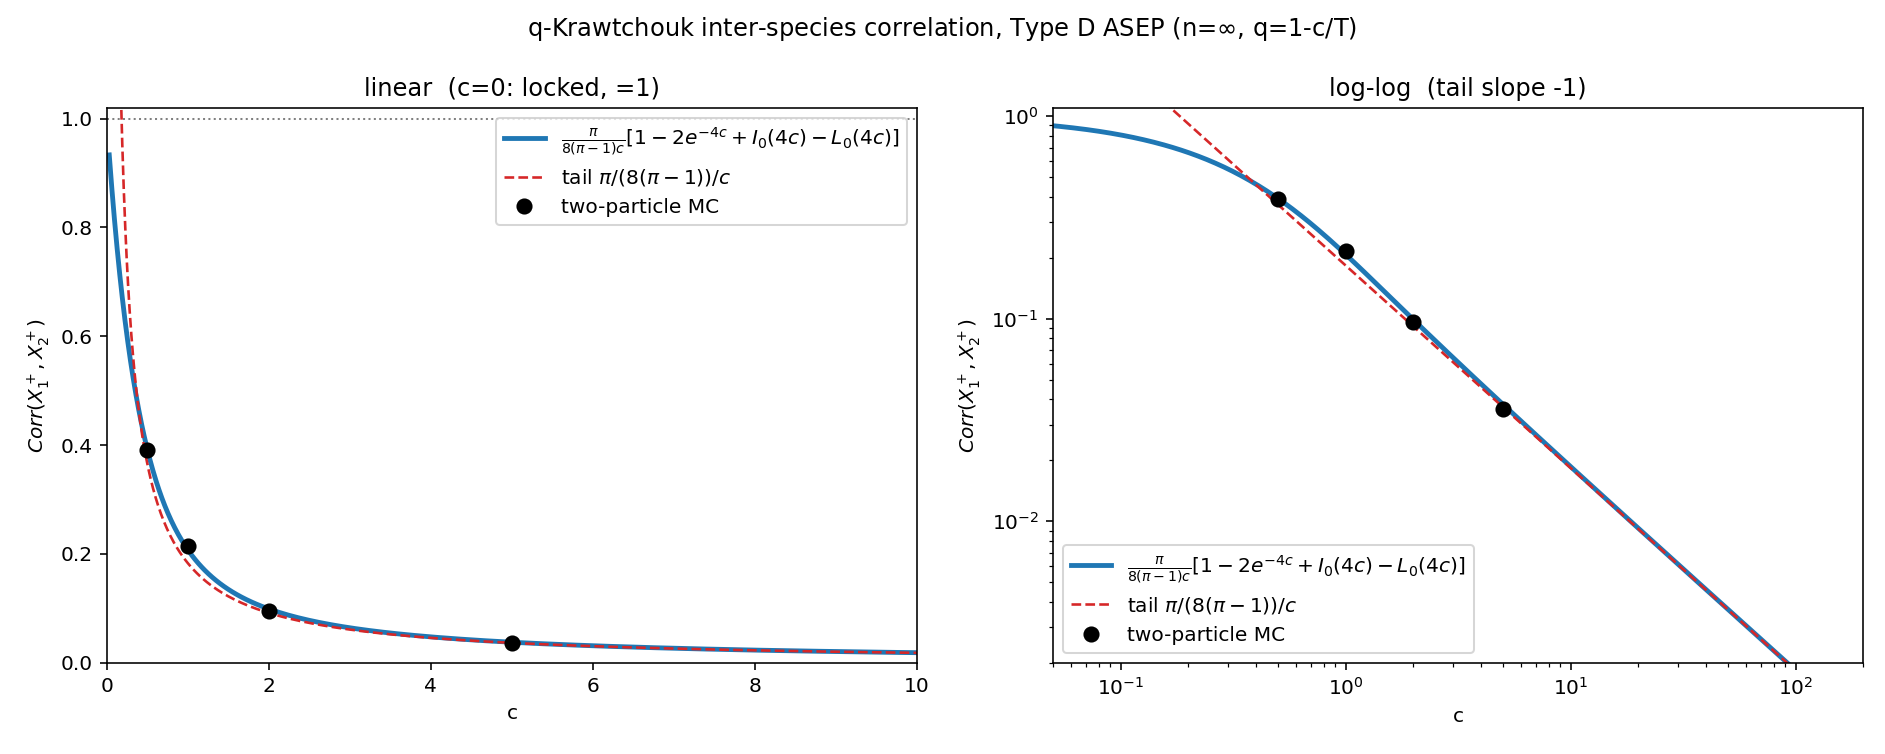
\includegraphics[width=0.49\textwidth]{corr_Xplus_c.png}\hfill
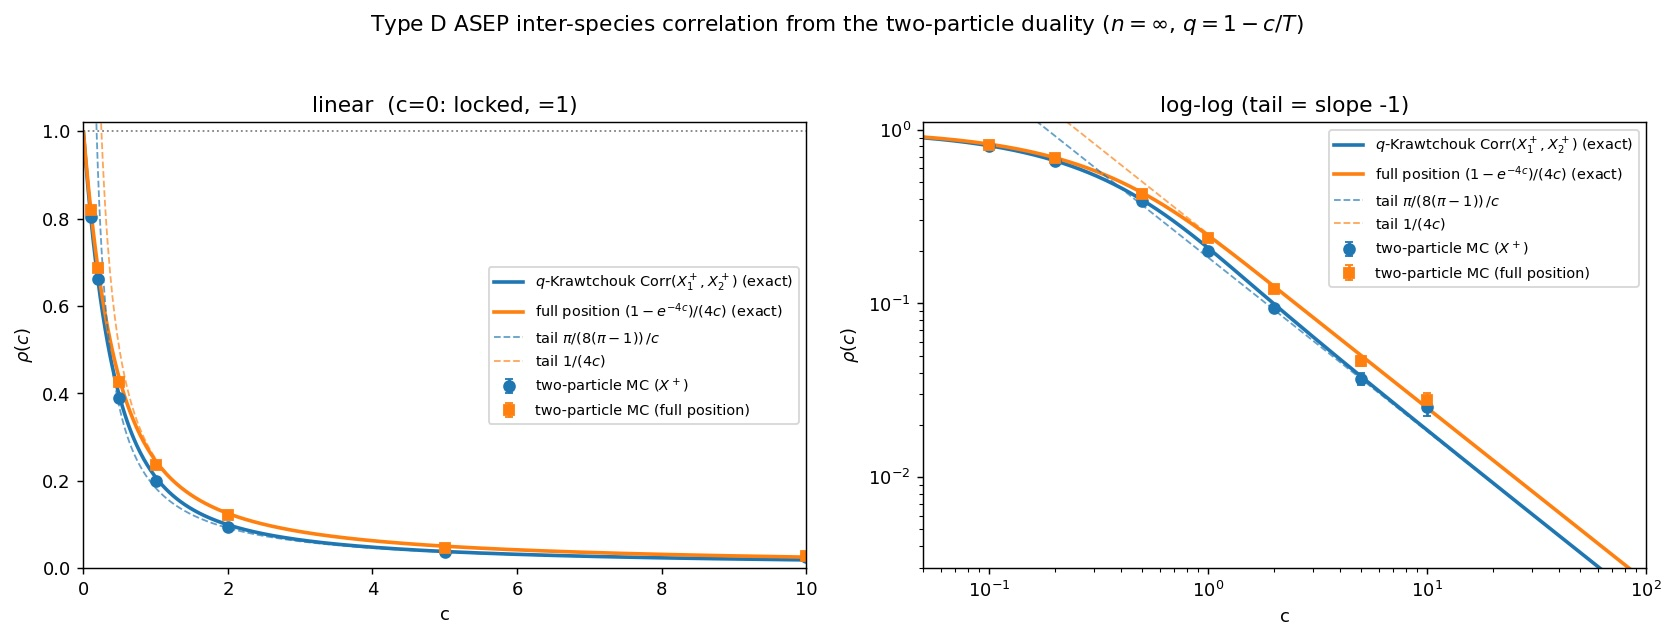
\includegraphics[width=0.49\textwidth]{rho_c_duality.jpg}
\caption{The initial--condition crossover of Theorem~\ref{thm:closed}. Left: the
one--sided observable $\Corr(X_1^+,X_2^+)$ (Bessel--Struve closed form, curve) against
two--particle Monte Carlo (dots), with the $\tfrac{\pi}{8(\pi-1)}c^{-1}$ tail. Right: the
full--position observable $\Corr(X_1,X_2)\to(1-e^{-4c})/(4c)$ against Monte Carlo. Both
run from perfectly correlated data ($\Corr\to1$ as $c\to0$) to the decoupled $1/c$ tail.}
\label{fig:rho}
\end{figure}

\subsection{The Tracy--Widom regime}
The covariance scales as $\Cov(N_1,N_2)\sim T^{1/2}$ (Conjecture~\ref{conj:cov}), confirmed
by exact augmented--matrix occupation--time computation ($\tau_0\sim T^{0.505}$,
$\Cov\sim T^{0.504}$ at $q=\tfrac12$) and by forward simulation
(Figure~\ref{fig:cov}, left). A dedicated forward run ($4.5\times10^4$ trials,
$T\le800$, $q=\tfrac12$) pins the prefactor: $\Cov(N_1,N_2)=(0.099\pm0.003)\sqrt T$,
in agreement with the $n=\infty$ data of Figure~\ref{fig:cov} ($\approx0.105\sqrt T$
over $T\in[10^2,10^4]$); the same run reproduces the Borodin--Corwin--Sasamoto
variance $2^{-8/3}(\gamma T)^{2/3}\Var(\chi_2)$, $\gamma=1-q^2$, to within $10\%$, and
exact integration of the relative--walk master equation gives
$\tau_0/\tau_1\to q^{-2}$ as in Proposition~\ref{prop:occ}. Both theoretical
candidate prefactors of Remark~\ref{rem:covconst} are excluded, so the constant
carries a nontrivial front factor. The marginals converge to $F_2$ (Figure~\ref{fig:cov},
middle: CDF/histogram; skewness $\to-0.21$, excess kurtosis $\to0.09$, the GUE
Tracy--Widom values), and the limit is $n$--independent (Figure~\ref{fig:cov}, right:
$n=2$ and $n=13$ collapse onto $F_2$). The standardised correlation accordingly decays,
$\Corr(N_1,N_2)\sim s^{-1/6}\to0$, the asymptotic decoupling of
Conjecture~\ref{conj:cov}.

\begin{figure}[h]\centering
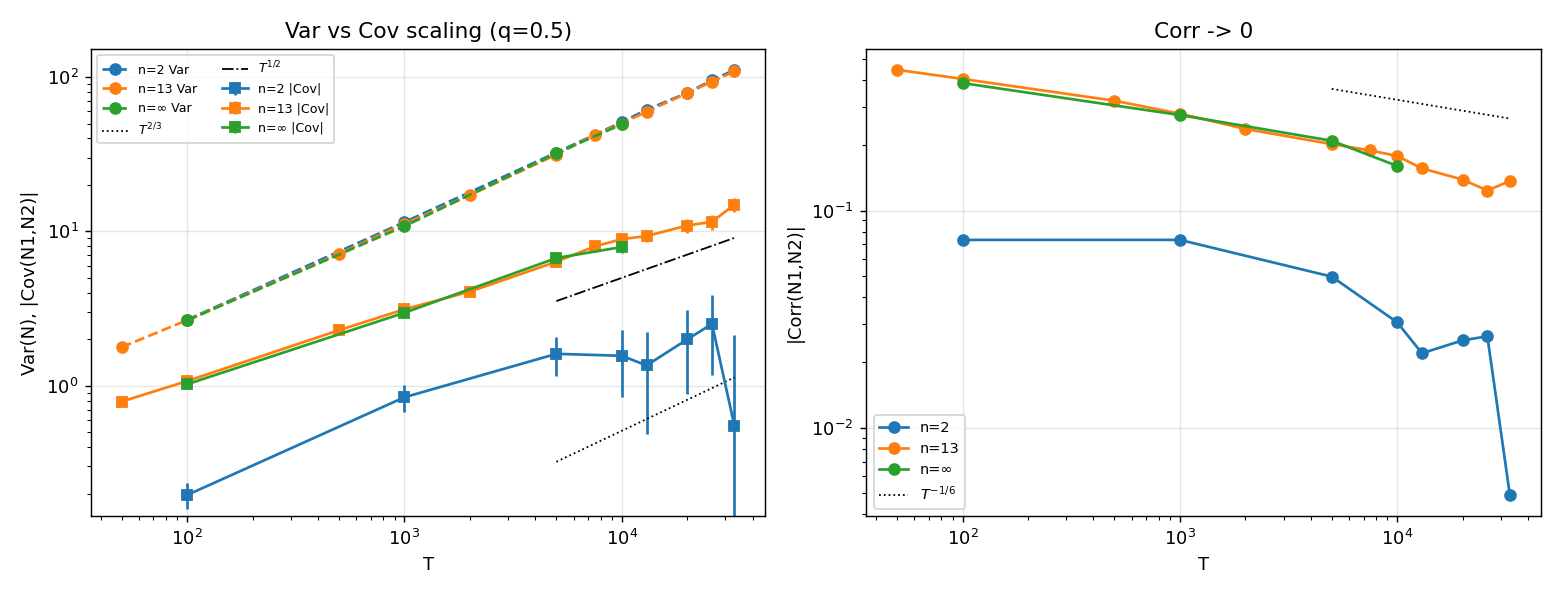
\includegraphics[width=0.32\textwidth]{cov_scaling_typeD.png}\hfill
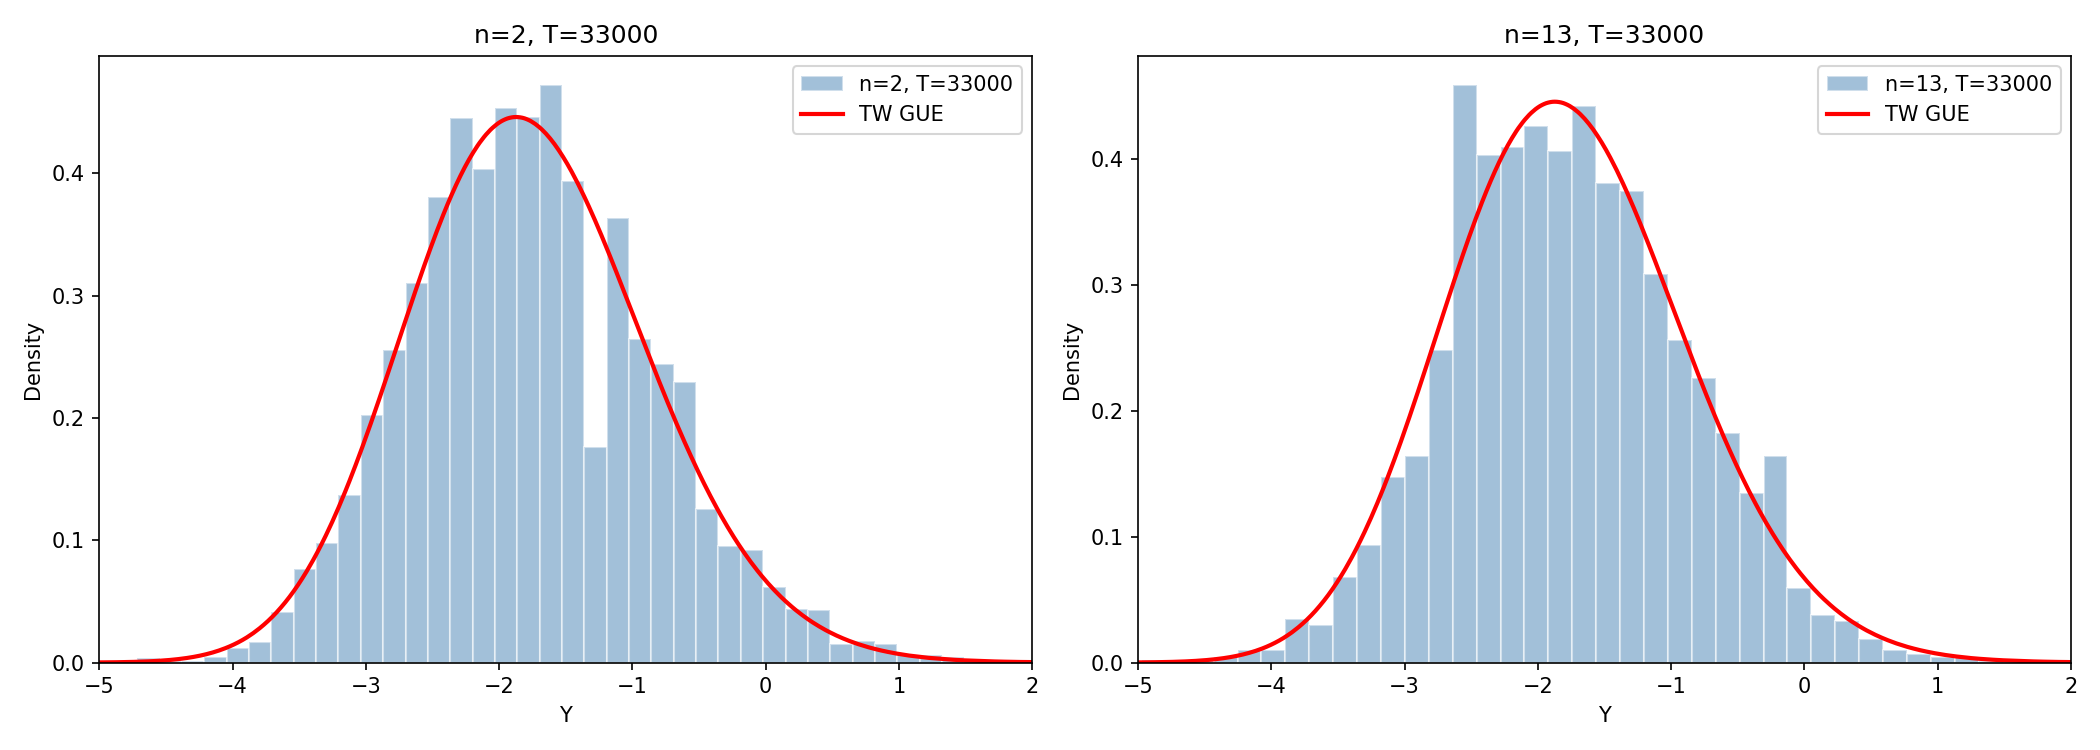
\includegraphics[width=0.32\textwidth]{histogram_vs_tw_T33000.png}\hfill
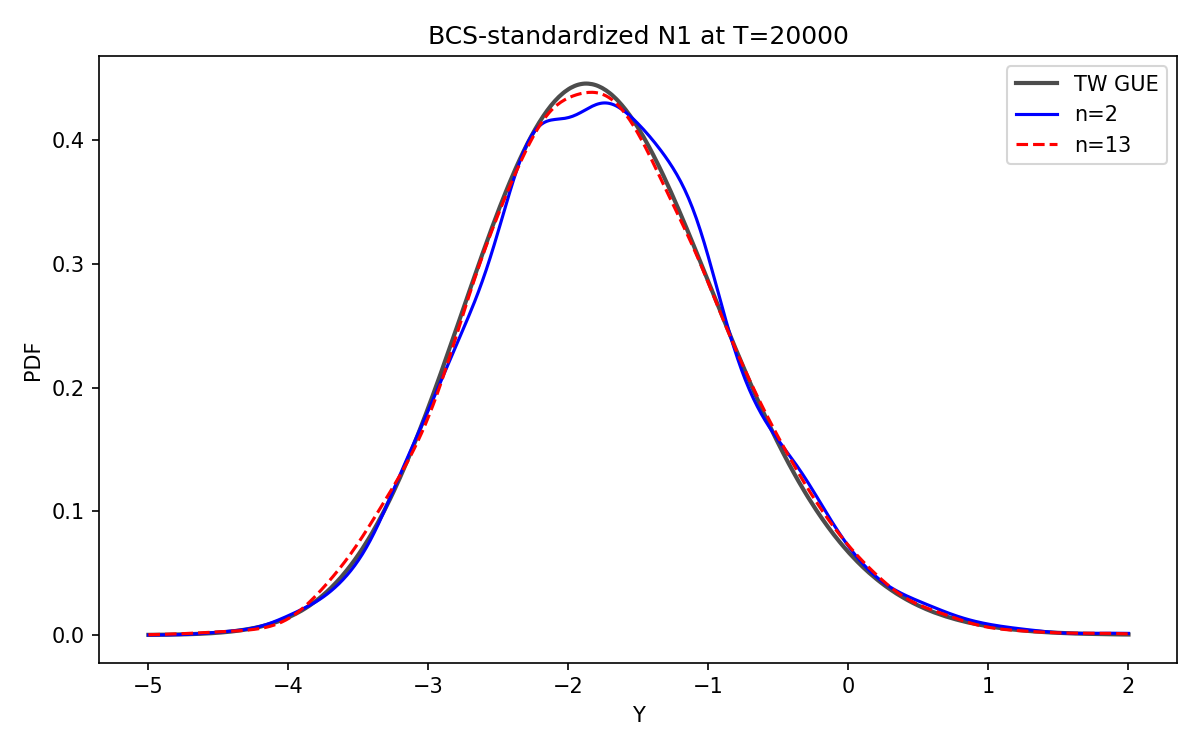
\includegraphics[width=0.32\textwidth]{n2_vs_n13_vs_tw_T20000.png}
\caption{The Tracy--Widom regime. Left: $\Cov(N_1,N_2)\sim T^{1/2}$, the uncorrelatedness
of Conjecture~\ref{conj:cov}. Middle: the marginal current against the GUE Tracy--Widom law
$F_2$ at $T=3.3\times10^4$. Right: $n$--independence --- the standardised marginals at
$n=2$ and $n=13$ collapse onto $F_2$.}
\label{fig:cov}
\end{figure}

\section{Discussion}\label{sec:disc}

The type D bound pair is a slow, near--conserved internal mode, yet in both scaling
regimes the species decouple in the limit, for one structural reason
(Remark~\ref{rem:transport}): the asymmetry lives only in the marginals
(Proposition~\ref{prop:decouple}), and the coupling is invisible to both equilibrium
transport coefficients (Proposition~\ref{prop:cross}). What is left of the coupling is a
transient, initial--condition--driven object: in regime (A) the entire crossover
$\rho(c)$ (Theorem~\ref{thm:closed}); in regime (B) the contact kernel of the exact
$q$--Laplace representation (Theorem~\ref{thm:cov}) and, conjecturally, the
sub--leading $s^{-1/6}$ correlation that decays to leave the two currents
uncorrelated (Conjecture~\ref{conj:cov}).
The two regimes are governed by one object --- the contact occupations
$(1+q^4)\tau_0-q^2\tau_{\pm1}$ of the relative walk --- in two
windows: at $\alpha=1$ the split rate is
$O(\eps)\to0$, $\tau_0=\Theta(T)$, the crossover $O(1)$; at $\alpha=0$ the split rate
is $\Theta(1)$, $\tau_0=\Theta(\sqrt T)$, the correlation sub--leading.

We emphasise the scope: both results are statements of \emph{decoupling}. In regime~(A)
the Gaussian limiting fields are uncoupled in drift and noise; in regime~(B) the two
currents decouple exactly at the level of the joint $q$--Laplace observable, and ---
conjecturally, with exact numerical scaling --- are asymptotically uncorrelated. We
do not address the finer question of whether the regime~(B) limit is a \emph{product}
(joint) law; the higher--order joint structure of the two currents, the linear
covariance asymptotics of Conjecture~\ref{conj:cov}, and its constant $c(q)$ are
facets of one open problem: the joint $q$--moment tower beyond two dual particles.

The Edwards--Wilkinson decoupling holds at \emph{arbitrary} densities $(\rho_1,\rho_2)$,
not only on the symmetric line (Theorem~\ref{thm:ewmain}): every ingredient is
density--free --- the current decoupling (Proposition~\ref{prop:decouple}), the
cross--noise cancellation $\E_\nu[V_x]=0$ (Proposition~\ref{prop:cross}), the
orthogonality $V_x\perp$ density (Lemma~\ref{lem:orth}), and the kernel bound
(Theorem~\ref{thm:kernel}), while the diagonal noise is per species --- so the two
fields decouple into linear stochastic heat equations with species--dependent noise
intensities $\sqrt{2\chi_iD}$, $\chi_i=\rho_i(1-\rho_i)$, and the bound--pair mode never
produces a third hydrodynamic field (Corollary~\ref{prop:sym}, Remark~\ref{rem:offline}).
The one genuinely open direction is the non--stationary EW analysis from block initial
data, for which $\rho(c)$ is the exact limiting cross--correlation and
Proposition~\ref{prop:twophase} the natural tool.

\paragraph{Status.} The $n=\infty$ self--duality is Theorem~\ref{thm:dual}(ii)
(two--site interlacing verified by computer algebra, extended to all $L$ by the
induction of \cite{REU}). The computer--algebra and numerical verifications cited in
Theorem~\ref{thm:dual}, Proposition~\ref{prop:decouplen}, Remark~\ref{rem:orthstatus},
Lemmas~\ref{lem:orth}, \ref{lem:eps} and \ref{lem:tridual}, and \S\ref{sec:numerics}
are reproduced by scripts to be included as ancillary files. In regime (A): Propositions~\ref{prop:cross},
\ref{prop:drift}, Corollary~\ref{prop:sym}, Lemmas~\ref{lem:orth}, \ref{lem:eqvar},
\ref{lem:free}--\ref{lem:tau}, \ref{lem:asep}, \ref{lem:split}, \ref{lem:rebind},
Theorems~\ref{thm:kernel}, \ref{thm:closed} and Proposition~\ref{prop:twophase} are
complete and self--contained; Proposition~\ref{prop:conc} rests on the exact,
machine--verified orthogonality relation \eqref{eq:orthexact} and is complete modulo
Lemma~\ref{lem:eps} (the dressed--mass estimate, perturbative and numerically
supported) and the infinite--volume step recorded in Remark~\ref{rem:orthstatus}; Theorem~\ref{thm:ewmain} is complete modulo the classical
single--species WASEP fluctuation result (used for the drift via
Proposition~\ref{prop:decouple} and the diagonal noise) and the classical
tightness/uniqueness \cite{KL}. In regime
(B): Theorem~\ref{thm:marg} (marginals, every $n$, via
Proposition~\ref{prop:decouplen}) is complete; Theorem~\ref{thm:cov} ($q$--Laplace
decoupling) is complete at $n=\infty$ --- the triangular reduction is
Lemma~\ref{lem:tridual} --- extends to $n=2,3$ via \cite{REU}, and for other finite
$n$ rests on the duality conjecture of \cite[Rmk.~4]{REU}; the linear--current
statement is Conjecture~\ref{conj:cov}, its constant open
(Remark~\ref{rem:covconst}). Section~\ref{sec:phase} is numerical/exploratory and frames the rigorous
results within the $(\alpha,q,n)$ picture.

\begin{thebibliography}{99}
\bibitem{ACR} M.~Ayala, G.~Carinci, F.~Redig, \emph{Quantitative Boltzmann--Gibbs
principles via orthogonal polynomial duality}, J.~Stat.~Phys.~\textbf{171} (2018),
980--999; arXiv:1712.08492.
\bibitem{ACR2} M.~Ayala, G.~Carinci, F.~Redig, \emph{Higher order fluctuation fields and
orthogonal duality polynomials}, Electron.~J.~Probab.~\textbf{26} (2021), 1--35;
arXiv:2004.08412.
\bibitem{REU} D.~Blyschak, O.~Burke, J.~Kuan, D.~Li, S.~Ustilovsky, Z.~Zhou,
\emph{Orthogonal polynomial duality of a two--species asymmetric exclusion process},
J.~Stat.~Phys.~\textbf{190} (2023), Paper No.~101; arXiv:2209.11114.
\bibitem{BCS} A.~Borodin, I.~Corwin, T.~Sasamoto, \emph{From duality to determinants for
$q$--TASEP and ASEP}, Ann.~Probab.~\textbf{42} (2014), 2314--2382; arXiv:1207.5035.
\bibitem{CFG20} G.~Carinci, C.~Franceschini, W.~Groenevelt, \emph{$q$-orthogonal
dualities for asymmetric particle systems}, Electron.~J.~Probab.~\textbf{26} (2021),
1--38; arXiv:2003.07837.
\bibitem{CKS} E.~A.~Carlen, S.~Kusuoka, D.~W.~Stroock, \emph{Upper bounds for symmetric
Markov transition functions}, Ann.~Inst.~H.~Poincar\'e Probab.~Statist.~\textbf{23}
(1987), suppl., 245--287.
\bibitem{CGRS} G.~Carinci, C.~Giardin\`a, F.~Redig, T.~Sasamoto, \emph{A generalized
asymmetric exclusion process with $U_q(\sutwo)$ stochastic duality}, Probab.~Theory
Related Fields \textbf{166} (2016), 887--933; arXiv:1407.3367.
\bibitem{EK} S.~N.~Ethier, T.~G.~Kurtz, \emph{Markov Processes: Characterization and
Convergence}, Wiley, 1986.
\bibitem{GJ} P.~Gon\c{c}alves, M.~Jara, \emph{Nonlinear fluctuations of weakly asymmetric
interacting particle systems}, Arch.~Ration.~Mech.~Anal.~\textbf{212} (2014), 597--644;
arXiv:1309.5120.
\bibitem{GJS} P.~Gon\c{c}alves, M.~Jara, M.~Simon, \emph{Second order Boltzmann--Gibbs
principle for polynomial functions and applications}, J.~Stat.~Phys.~\textbf{166} (2017),
90--113; arXiv:1507.06076.
\bibitem{Groenevelt} W.~Groenevelt, \emph{Orthogonal stochastic duality functions from Lie
algebra representations}, J.~Stat.~Phys.~\textbf{174} (2019), 97--119; arXiv:1709.05997.
\bibitem{KLLPZ} J.~Kuan, M.~Landry, A.~Lin, A.~Park, Z.~Zhou, \emph{Interacting particle
systems with type D symmetry and duality}, arXiv:2011.13473.
\bibitem{KL} C.~Kipnis, C.~Landim, \emph{Scaling Limits of Interacting Particle Systems},
Grundlehren \textbf{320}, Springer, 1999.
\bibitem{LawlerLimic} G.~F.~Lawler, V.~Limic, \emph{Random Walk: A Modern Introduction},
Cambridge Stud.~Adv.~Math.~\textbf{123}, Cambridge Univ.~Press, 2010.
\bibitem{Petrov} V.~V.~Petrov, \emph{Sums of Independent Random Variables}, Springer, 1975.
\bibitem{Price} R.~Price, \emph{A useful theorem for nonlinear devices having Gaussian
inputs}, IRE Trans.~Inform.~Theory \textbf{4} (1958), 69--72.
\bibitem{RSL} E.~Rohr, K.~Sellakumaran Latha, A.~Yin, \emph{A type D asymmetric simple
exclusion process generated by an explicit central element of
$\mathcal U_q(\so_{10})$}, arXiv:2307.15660.
\bibitem{Schutz} G.~M.~Sch\"utz, \emph{Exact solution of the master equation for the
asymmetric exclusion process}, J.~Stat.~Phys.~\textbf{88} (1997), 427--445.
\bibitem{Sheppard} W.~F.~Sheppard, \emph{On the application of the theory of error to cases
of normal distribution and normal correlation}, Phil.~Trans.~R.~Soc.~A \textbf{192}
(1899), 101--167.
\end{thebibliography}

\end{document}
